% ****** Start of file apssamp.tex ******
\documentclass[%
reprint,
amsmath,amssymb,
aps,
]{revtex4-2}

\usepackage{graphicx}
\usepackage{dcolumn}
\usepackage{bm}
\usepackage[utf8]{inputenc} 
\usepackage[T1]{fontenc}    
\usepackage[spanish]{babel} 
\usepackage[colorlinks=true, linkcolor=blue, citecolor=blue, urlcolor=blue]{hyperref}

\decimalpoint

\begin{document}
	
	\title{Efectos de la topología en el modelo SIS}
	
	\author{Javier Campos Vallejo}
	\affiliation{Universidad de Granada}
	\author{Eugenio Etcheverría Sanz}
	\affiliation{Universidad de Granada}
	
	\date{\today}
	
	\begin{abstract}
		% Aquí irá tu resumen
	\end{abstract}
	
	\maketitle
	
	\section{\label{sec:introduccion}Introducción}
	El estudio de la propagación de epidemias en el marco de la Física de los Sistemas Complejos es crucial para comprender los mecanismos relacionados que determinan la persistencia o la extinción de una enfermedad en una población. Más allá de su evidente interés epidemiológico, estos modelos constituyen buenos ejemplos de sistemas estocásticos dinámicos con transiciones de fase fuera del equilibrio. En particular, permiten explorar la criticidad universal intrínseca de la mecánica estadística, una propiedad fundamental que define el comportamiento del sistema cerca de su punto crítico y que será analizada en detalle en este trabajo.~\cite{PastorSatorras2015,Dorogovtsev2008,Albert2002,Odor2004}
	
	Entre los diversos marcos teóricos disponibles, este trabajo se centra en el modelo \textit{Susceptible-Infectado-Susceptible} (SIS). Este modelo describe dinámicas de contagio en las que los individuos infectados se recuperan a una cierta tasa, pero al hacerlo no adquieren inmunidad, volviendo a ser susceptibles de forma inmediata y pudiendo reiniciar el ciclo de contagios. Resulta especialmente adecuado para modelar infecciones con inmunidad efímera o inexistente, como el resfriado común.~\cite{PastorSatorras2015}
	
	
	El objetivo principal de este trabajo es investigar cómo la topología de las interacciones y la heterogeneidad estructural afectan al comportamiento crítico del modelo SIS. Mediante aproximaciones analíticas de campo medio y simulaciones estocásticas, se analizará la dinámica sobre distintas arquitecturas de red (Erdős-Rényi, Watts-Strogatz y  Barabási-Albert). A través de este análisis comparativo, se estudiará el desplazamiento y colapso del umbral epidémico, los exponentes críticos, y la eventual emergencia de dinámicas de relajación anómala (fases de Griffiths) dictadas por el desorden congelado.~\cite{Muñoz2010,Noest1986,Odor2004,Dorogovtsev2008,Roig2026}
	%El objetivo principal de este trabajo es investigar cómo la topología de las redes de interacción y la heterogeneidad estructural afectan al comportamiento crítico del modelo SIS. Mediante aproximaciones analíticas de campo medio y simulaciones estocásticas sobre distintas arquitecturas de red, se analizará el desplazamiento del umbral epidémico, la alteración de los exponentes críticos y la eventual emergencia de dinámicas dictadas por el desorden topológico.
	
	\section{Definición del Modelo y Variables}
	El modelo SIS asume una población total constante $N$, donde los individuos pueden estar en dos estados diferentes:
	\begin{itemize}
		\item \textbf{Susceptibles ($S$):} Individuos sanos que pueden contraer la enfermedad.
		\item \textbf{Infectados ($I$):} Individuos enfermos que pueden transmitir la enfermedad y que acaban sanando pero que no adquieren inmunidad, permitiendo la reinfección.
	\end{itemize}
	
	Como la población no varía con el tiempo, siempre se cumple que $S + I = N$. El objetivo de este estudio es analizar la evolución de la \textbf{densidad de infectados} ($\rho = I/N$).~\cite{PastorSatorras2015}
	
	\subsection{Tasas de Transición}\label{sec:tasas_trans}
	Definimos las tasas de transición macroscópicas $W(I \to I')$ que determinan la evolución del número total de infectados:
	
	\textbf{Tasa de Infección, $W(I \to I+1)$:} Un individuo infectado transmite la enfermedad con una tasa $\beta$. En un entorno bien mezclado, la probabilidad de que el contacto sea susceptible es $S/N$. Como hay $I$ personas infectadas, la tasa total es:
	\begin{equation}
		W(I \to I+1) = \beta I \frac{S}{N} = \beta I \frac{N - I}{N}
	\end{equation}
	
	\textbf{Tasa de Recuperación, $W(I \to I-1)$:} Cada individuo infectado se recupera con una tasa constante $\mu$. Para $I$ infectados, la tasa total es:
	\begin{equation}
		W(I \to I-1) = \mu I
	\end{equation}
	
	El modelo SIS está gobernado por las transiciones elementales:~\cite{PastorSatorras2015,Roig2026}
	\begin{align}
		S + I &\xrightarrow{\beta} 2I, \\
		I &\xrightarrow{\mu} S.
	\end{align}
	
	\section{Aproximación de Campo Medio a partir de la Ecuación Maestra}
	
	El sistema asume inicialmente un \textbf{entorno bien mezclado} (\textit{well-mixed environment}). Esto significa que asumimos que cualquier individuo tiene la misma probabilidad de interactuar con cualquier otro individuo de la población, ignorando la estructura topológica local de la red.~\cite{PastorSatorras2015,Dorogovtsev2008,Albert2002}
	
	
	
	\subsection{Evolución y Estado Estacionario}
	Aplicando la ecuación maestra y la aproximación de campo medio ($\langle I^2 \rangle \approx \langle I \rangle^2$, véase el desarrollo detallado en el Apéndice \ref{apendice:mean_field}), la evolución de la densidad de infectados viene dada por:
	\begin{equation}
		\frac{d\rho}{dt} = \beta \rho (1 - \rho) - \mu \rho
	\end{equation}
	
	Para encontrar el umbral crítico $\beta_c$, se analiza el estado estacionario ($d\rho/dt = 0$), obteniendo dos soluciones: el estado libre de enfermedad ($\rho^* = 0$) y el estado endémico ($\rho^* = 1 - \mu/\beta$). El intercambio de estabilidad entre ambas soluciones define una bifurcación transcrítica en el sistema (Fig. \ref{fig:bifurcacion}), estableciendo el umbral epidémico clásico:~\cite{PastorSatorras2015}
	\begin{equation}
		\beta_c = \mu
	\end{equation}
	Este valor representa la tasa macroscópica global. A nivel microscópico, en una red homogénea de grado medio $\langle k \rangle$, la tasa crítica equivalente por enlace es $\beta_c^{micro} = \mu / \langle k \rangle$.~\cite{PastorSatorras2015,Albert2002}
	
	\begin{figure}[htbp]
		\centering
		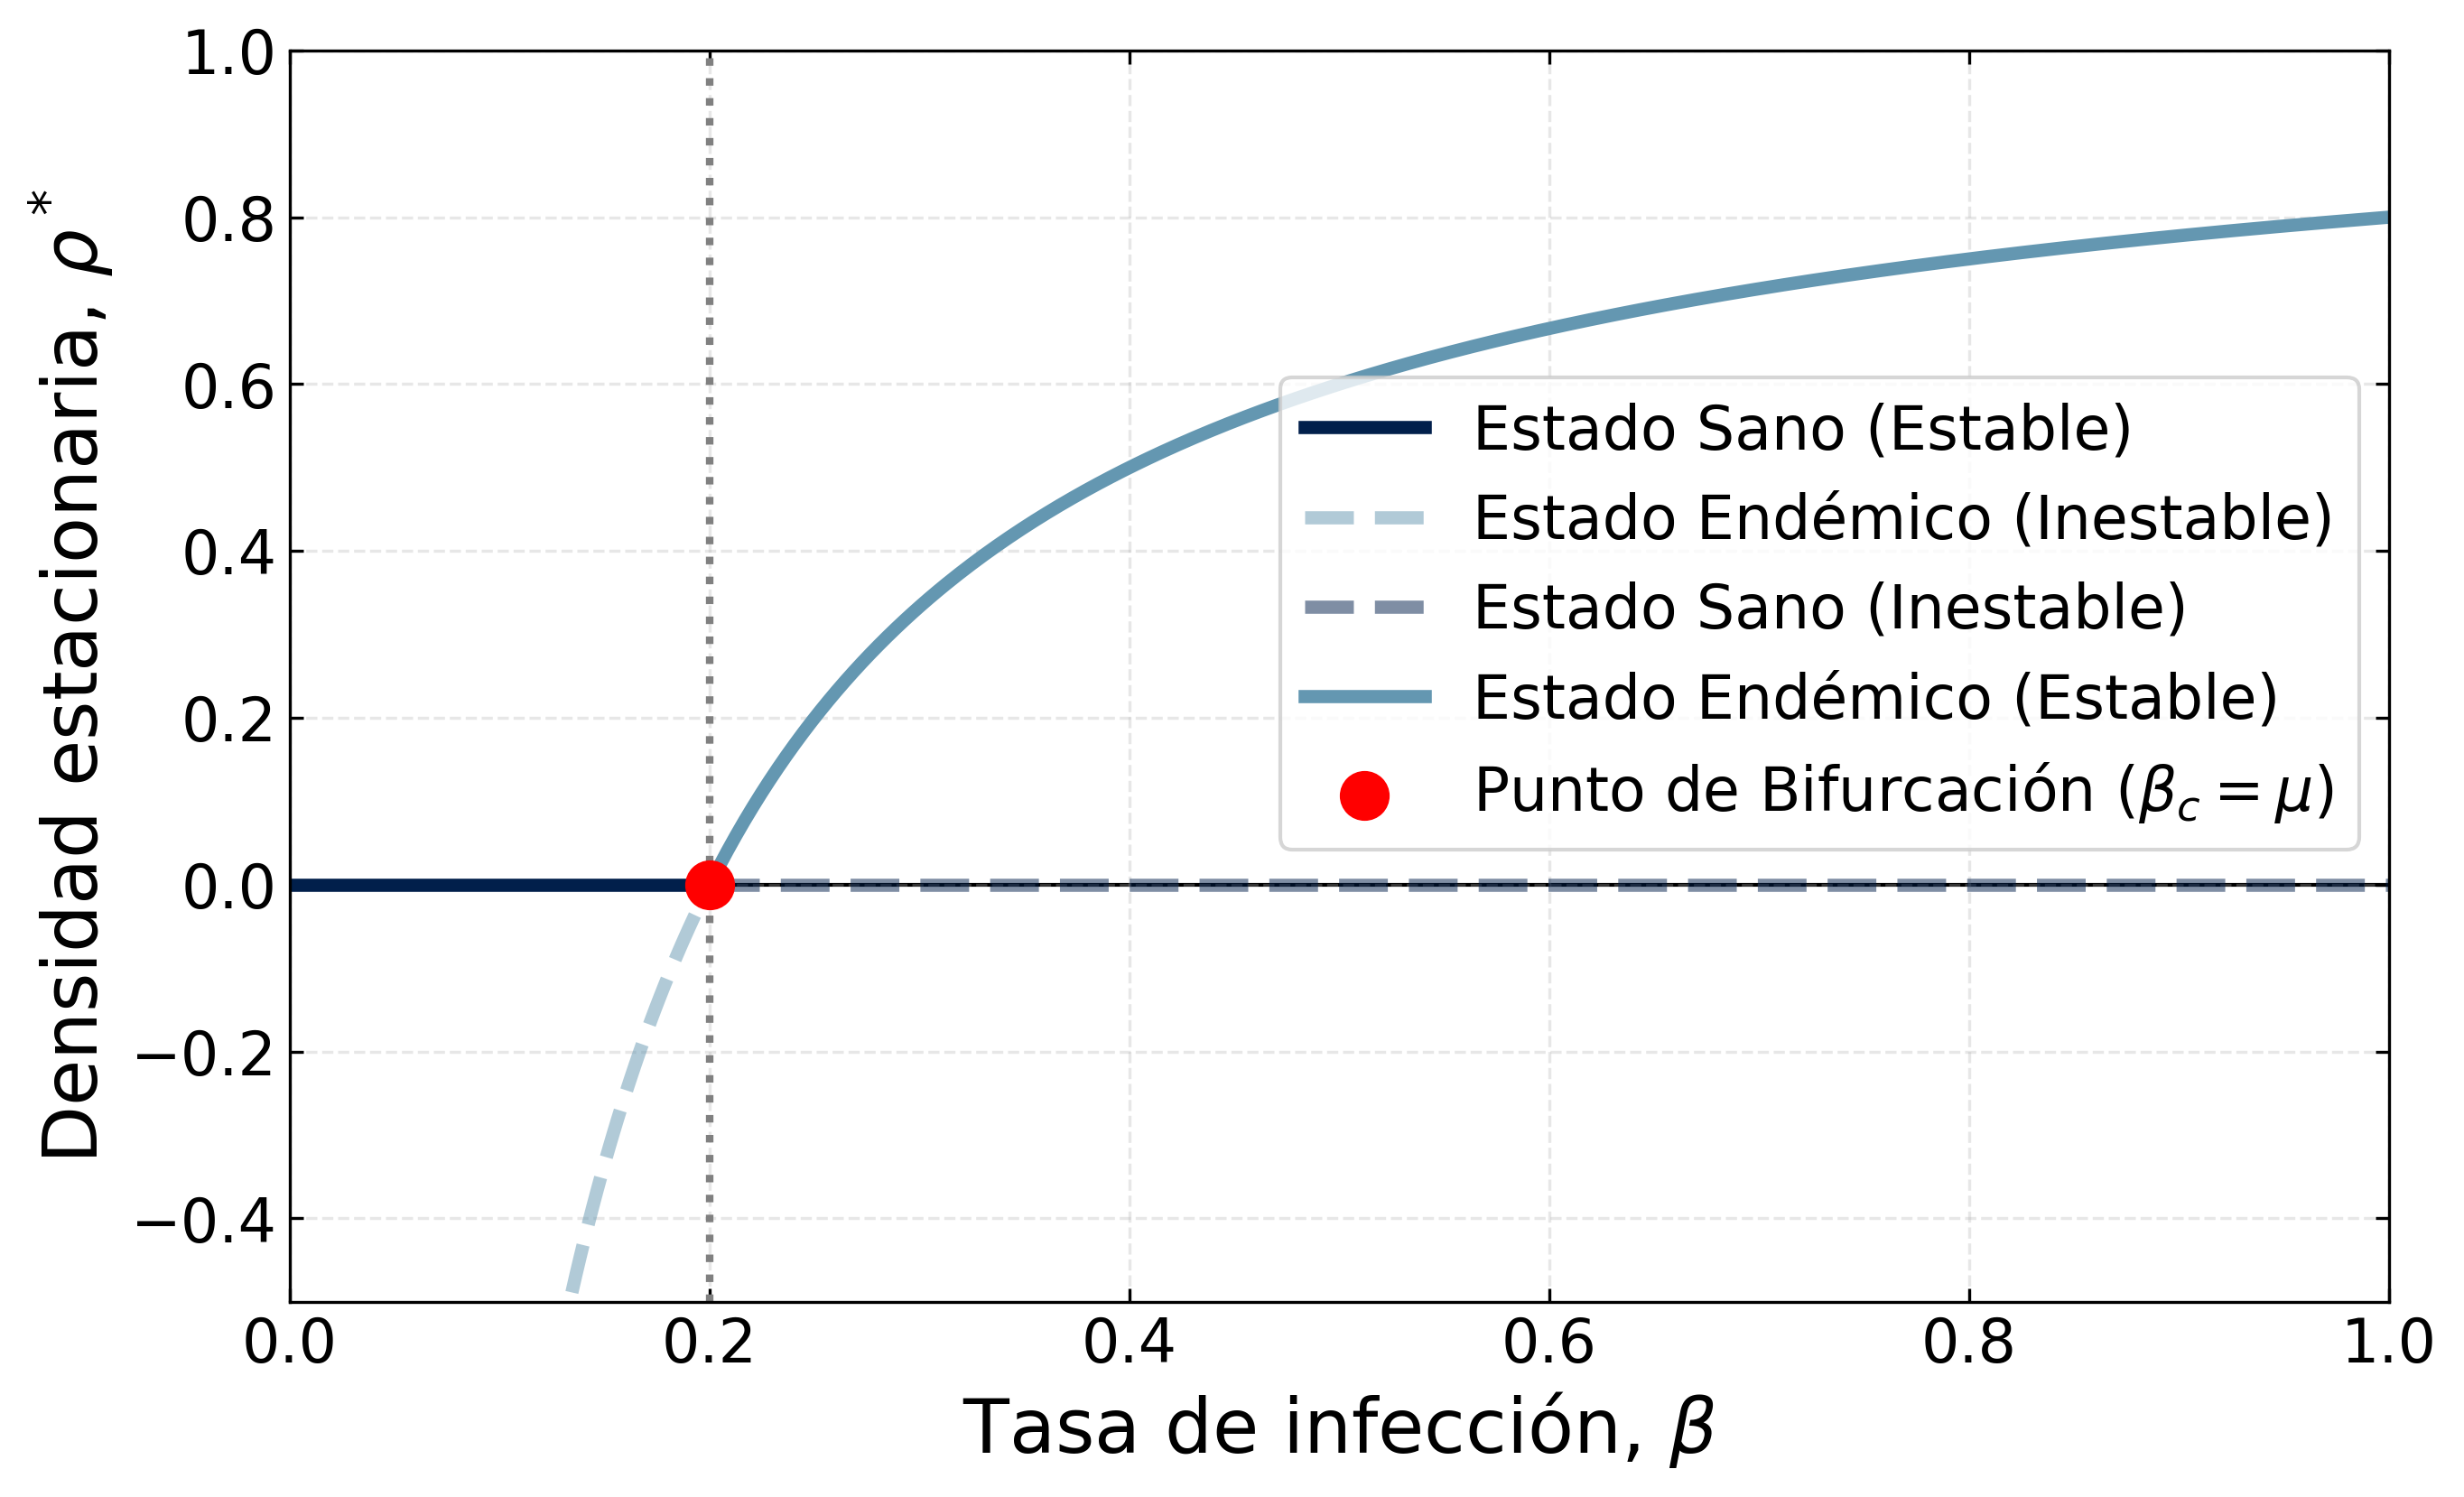
\includegraphics[width=0.9\columnwidth]{imagenes/Bifurcacion_SIS.png}
		\caption{Diagrama de bifurcación transcrítica en la aproximación de campo medio del modelo SIS. En $\beta_c = \mu$, la rama trivial pierde estabilidad en favor del estado endémico.}
		\label{fig:bifurcacion}
	\end{figure}
	
	\section{Aproximación DBMF en Redes Heterogéneas}
	La aproximación clásica asume homogeneidad en los contactos, lo cual no es realista para redes complejas donde algunos nodos (\textit{hubs}) tienen muchas más conexiones que otros.~\cite{Albert2002,Dorogovtsev2008,PastorSatorras2015} Empleando la aproximación \textit{Degree-Based Mean-Field} (DBMF), la red se divide en clases según su grado $k$.
	
	Definiendo $\rho_k(t)$ como la fracción de infectados entre los nodos de grado $k$, la evolución temporal se escribe como:
	\begin{equation}\label{ec:din_dbmf_het}
		\frac{d\rho_k(t)}{dt} = -\mu \rho_k(t) + \beta k [1 - \rho_k(t)] \Theta(\rho, t)
	\end{equation}
	donde $\Theta(\rho, t)$ es la probabilidad de que un enlace cualquiera apunte a un nodo infectado. En redes heterogéneas, al seguir un enlace al azar, existe una probabilidad estadísticamente mayor de desembocar en un \textit{hub}, lo cual captura la propensión de estos nodos a actuar como reservorios persistentes.
	
	Tras resolver el estado estacionario (Apéndice \ref{apendice:dbmf}), se demuestra que el umbral epidémico ($\lambda = \beta/\mu$) depende de los momentos de la distribución de grado:~\cite{PastorSatorras2015,Albert2002,Dorogovtsev2008,Roig2026}
	\begin{equation}
		\lambda_c = \frac{\langle k \rangle}{\langle k^2 \rangle}
		\label{eq:dbmf_threshold}
	\end{equation}
	
	Es importante notar que $\lambda_c = \beta_c/\mu$ representa el umbral crítico en unidades adimensionales. Por tanto, la tasa de infección crítica que se observa en las simulaciones se relaciona directamente mediante $\beta_c = \mu \lambda_c = \mu \frac{\langle k \rangle}{\langle k^2 \rangle}$.
	
	En redes de libre escala, el segundo momento $\langle k^2 \rangle$ diverge en el límite termodinámico, lo que implica que el umbral epidémico tiende a cero ($\lambda_c \to 0$).~\cite{PastorSatorras2015,Albert2002,Dorogovtsev2008}
	
	\section{Estudio Numérico de la Transición de Fase}
	
	Para contrastar las predicciones analíticas, se ha llevado a cabo un análisis numérico del modelo SIS mediante simulaciones de Monte Carlo. Las simulaciones se ejecutaron sobre tres arquitecturas canónicas: redes de Erdős-Rényi (ER), redes de pequeño mundo de Watts-Strogatz (WS) y redes libres de escala de Barabási-Albert (BA).~\cite{Albert2002,Dorogovtsev2008,PastorSatorras2015} Para caracterizar adecuadamente la transición, se estudiaron redes de hasta $N=500\,000$ nodos con una conectividad media fijada en $\langle k \rangle = 10$, manteniendo una tasa de recuperación constante $\mu = 0.2$ y una fracción de nodos infectados inicial del $10\%$.
	
	La Figura \ref{fig:time_ev} ilustra la evolución temporal de la densidad de infectados $\rho(t)$ para múltiples valores de la tasa de infección $\beta$. Se observa cómo, tras un régimen transitorio inicial, el sistema relaja hacia su estado estacionario.
	
	\begin{figure}[htbp]
		\centering
		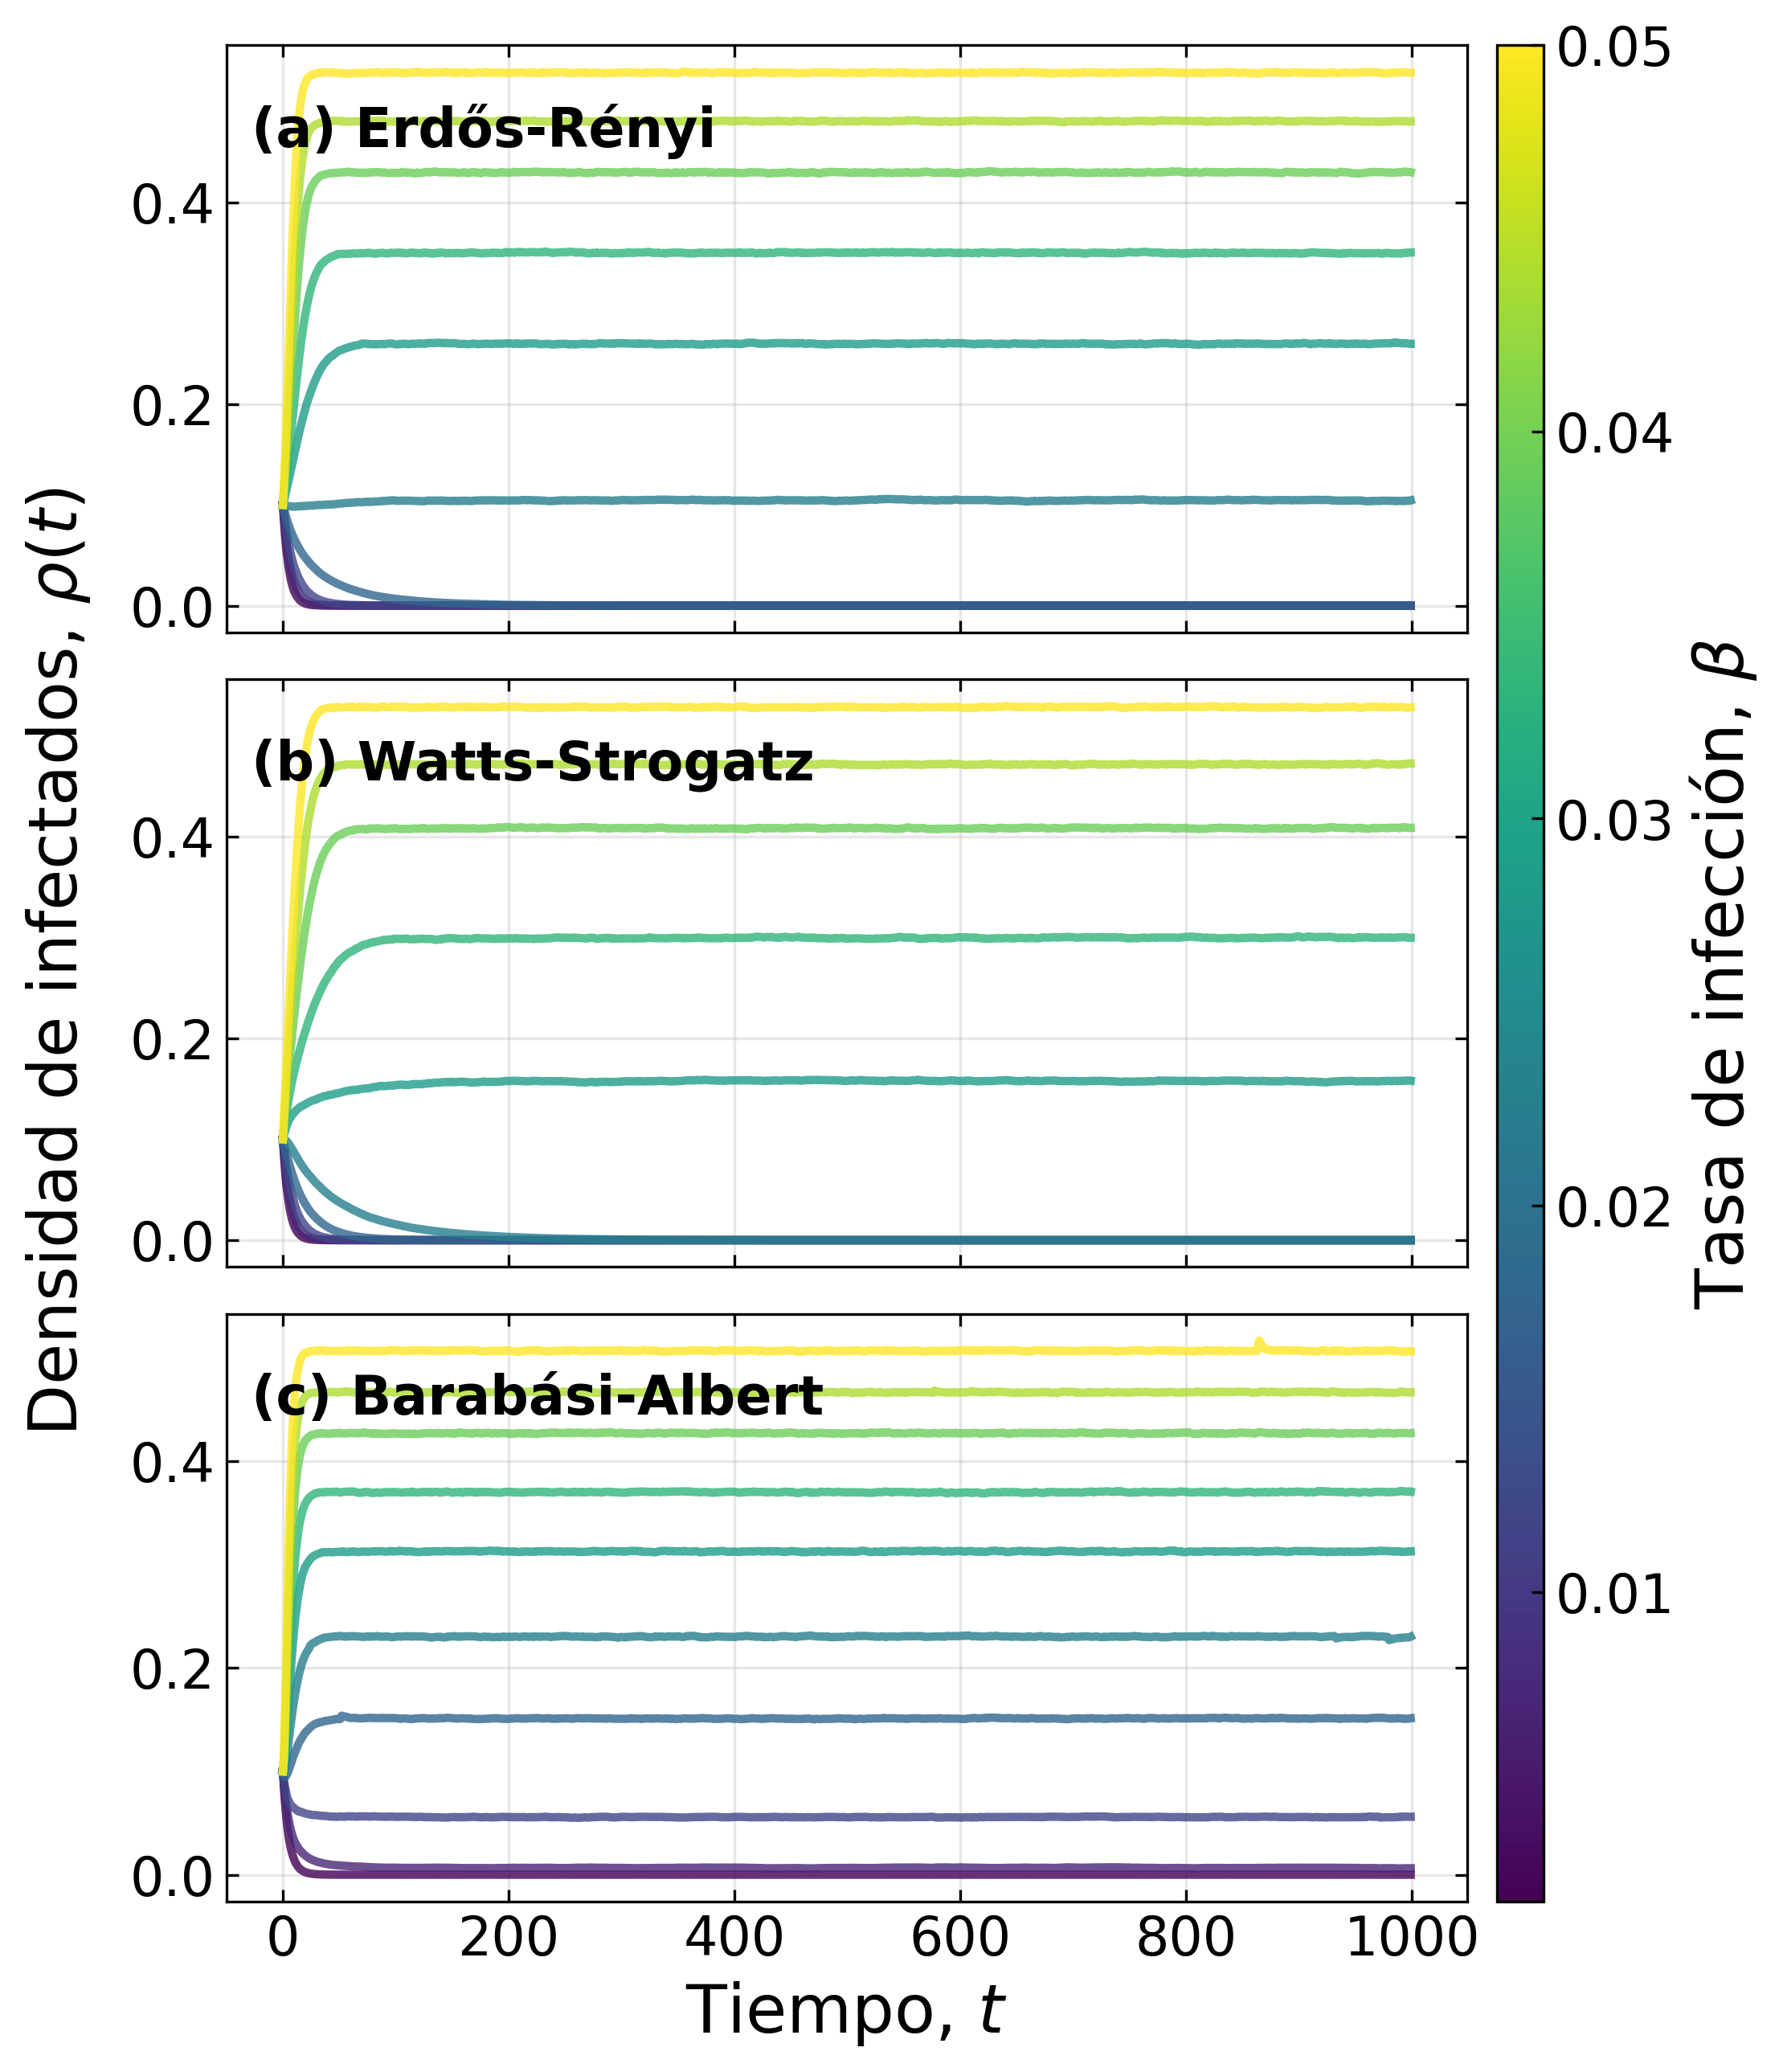
\includegraphics[width=\columnwidth]{imagenes/4_time_evolution_STACKED_N500000.png}
		\caption{Evolución temporal de la densidad de infectados $\rho(t)$ para redes de $N=500.000$ nodos. Se muestran diversas curvas correspondientes a diferentes tasas de infección $\beta$, evidenciando la estabilización del sistema tras el régimen transitorio.}
		\label{fig:time_ev}
	\end{figure}
	
	\subsection{Determinación del Umbral Epidémico y Susceptibilidad}
	
	La transición de fase epidémica puede observarse macroscópicamente al representar la densidad estacionaria de infectados $\langle \rho \rangle$ frente a $\beta$ (Fig. \ref{fig:phase_trans}). Las redes homogéneas (ER y WS) presentan un umbral claro de persistencia que concuerda excelentemente con las predicciones teóricas (Ec. \ref{eq:dbmf_threshold}). 
	
	\begin{figure}[htbp]
		\centering
		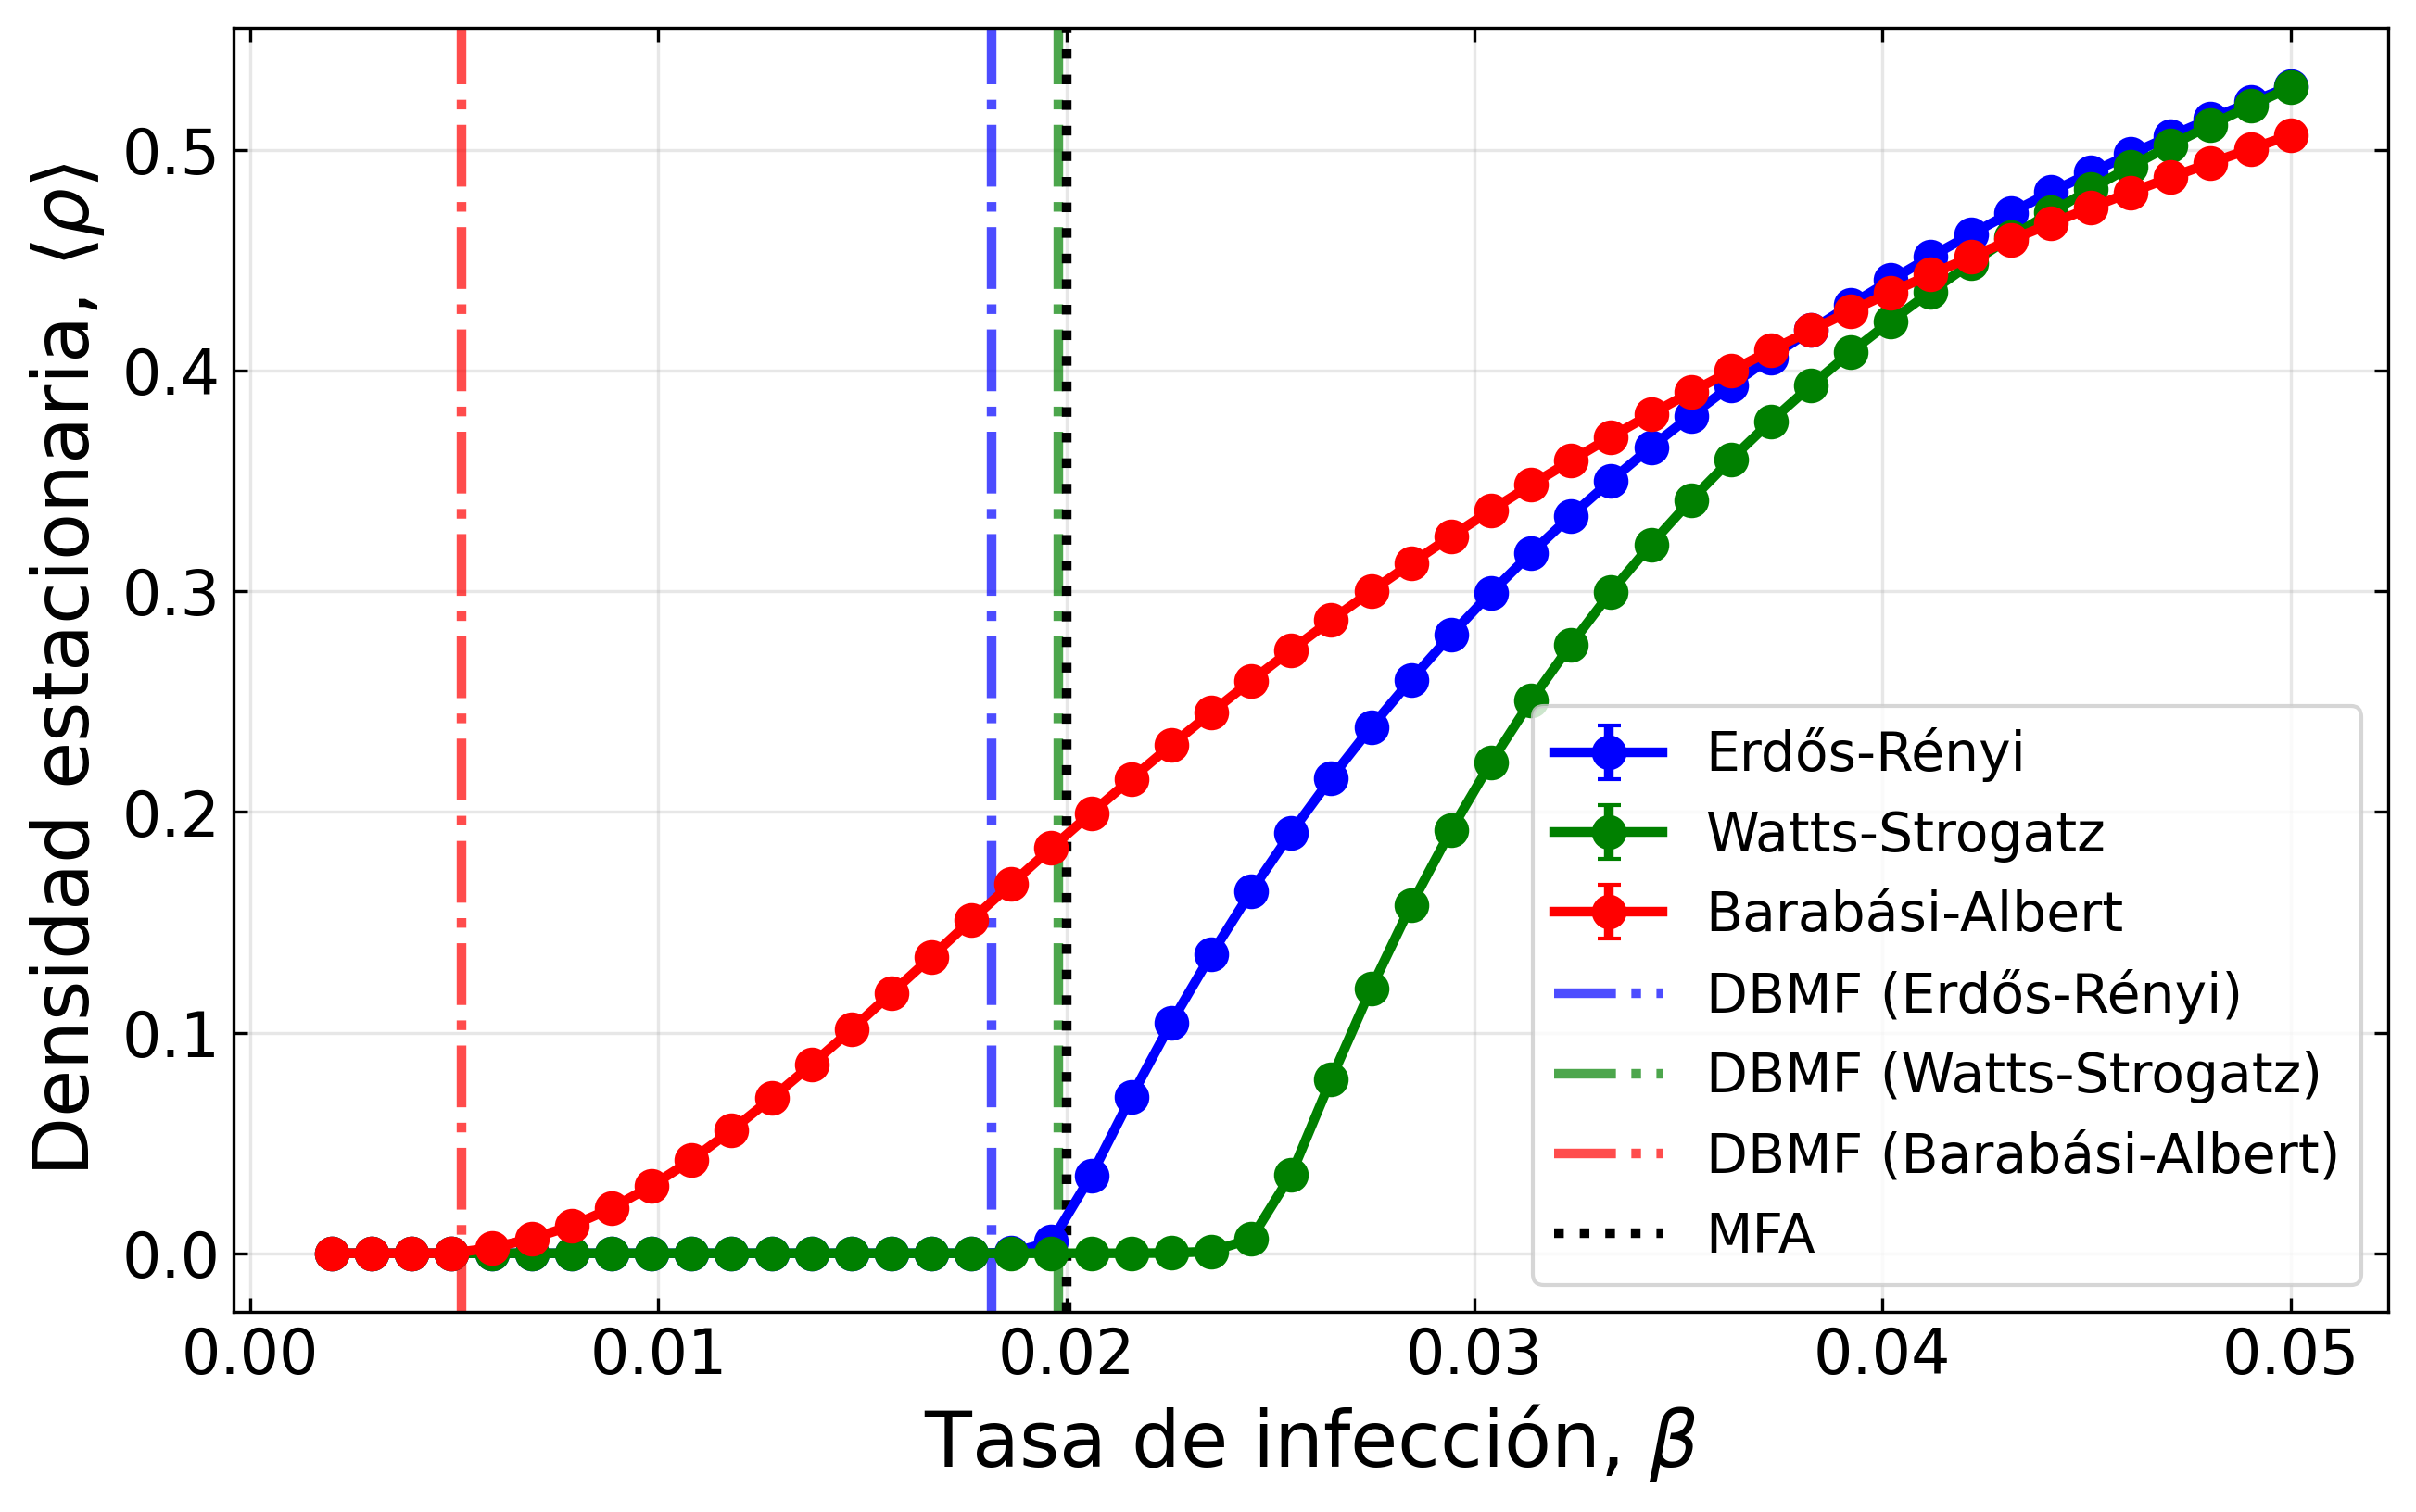
\includegraphics[width=\columnwidth]{imagenes/5_comparison_phase_transition_N500000.png}
		\caption{Diagrama de fases comparativo para la densidad estacionaria de infectados $\langle \rho \rangle$. Se superponen las líneas teóricas para la aproximación homogénea (MFA) y heterogénea (DBMF).}
		\label{fig:phase_trans}
	\end{figure}
	
	Para localizar con precisión el punto crítico $\beta_c$ en sistemas de tamaño finito, se recurre a la susceptibilidad del sistema, definida a través de las fluctuaciones del parámetro de orden en el estado estacionario~\cite{Roig2026}:
	\begin{equation}
		\chi = N (\langle \rho^2 \rangle - \langle \rho \rangle^2)
	\end{equation}
	
	Como se aprecia en la Figura \ref{fig:susc}, la susceptibilidad exhibe un pico divergente característico de las transiciones de fase continuas. El máximo de este pico proporciona la estimación numérica más robusta para $\beta_c(N)$. En la red de Barabási-Albert, la extrema heterogeneidad del grado suprime la transición abrupta, difuminando el pico de susceptibilidad y desplazando el inicio de la epidemia hacia el origen, confirmando el colapso del umbral epidémico predicho por DBMF.~\cite{PastorSatorras2015,Albert2002,Dorogovtsev2008}
	
	\begin{figure}[htbp]
		\centering
		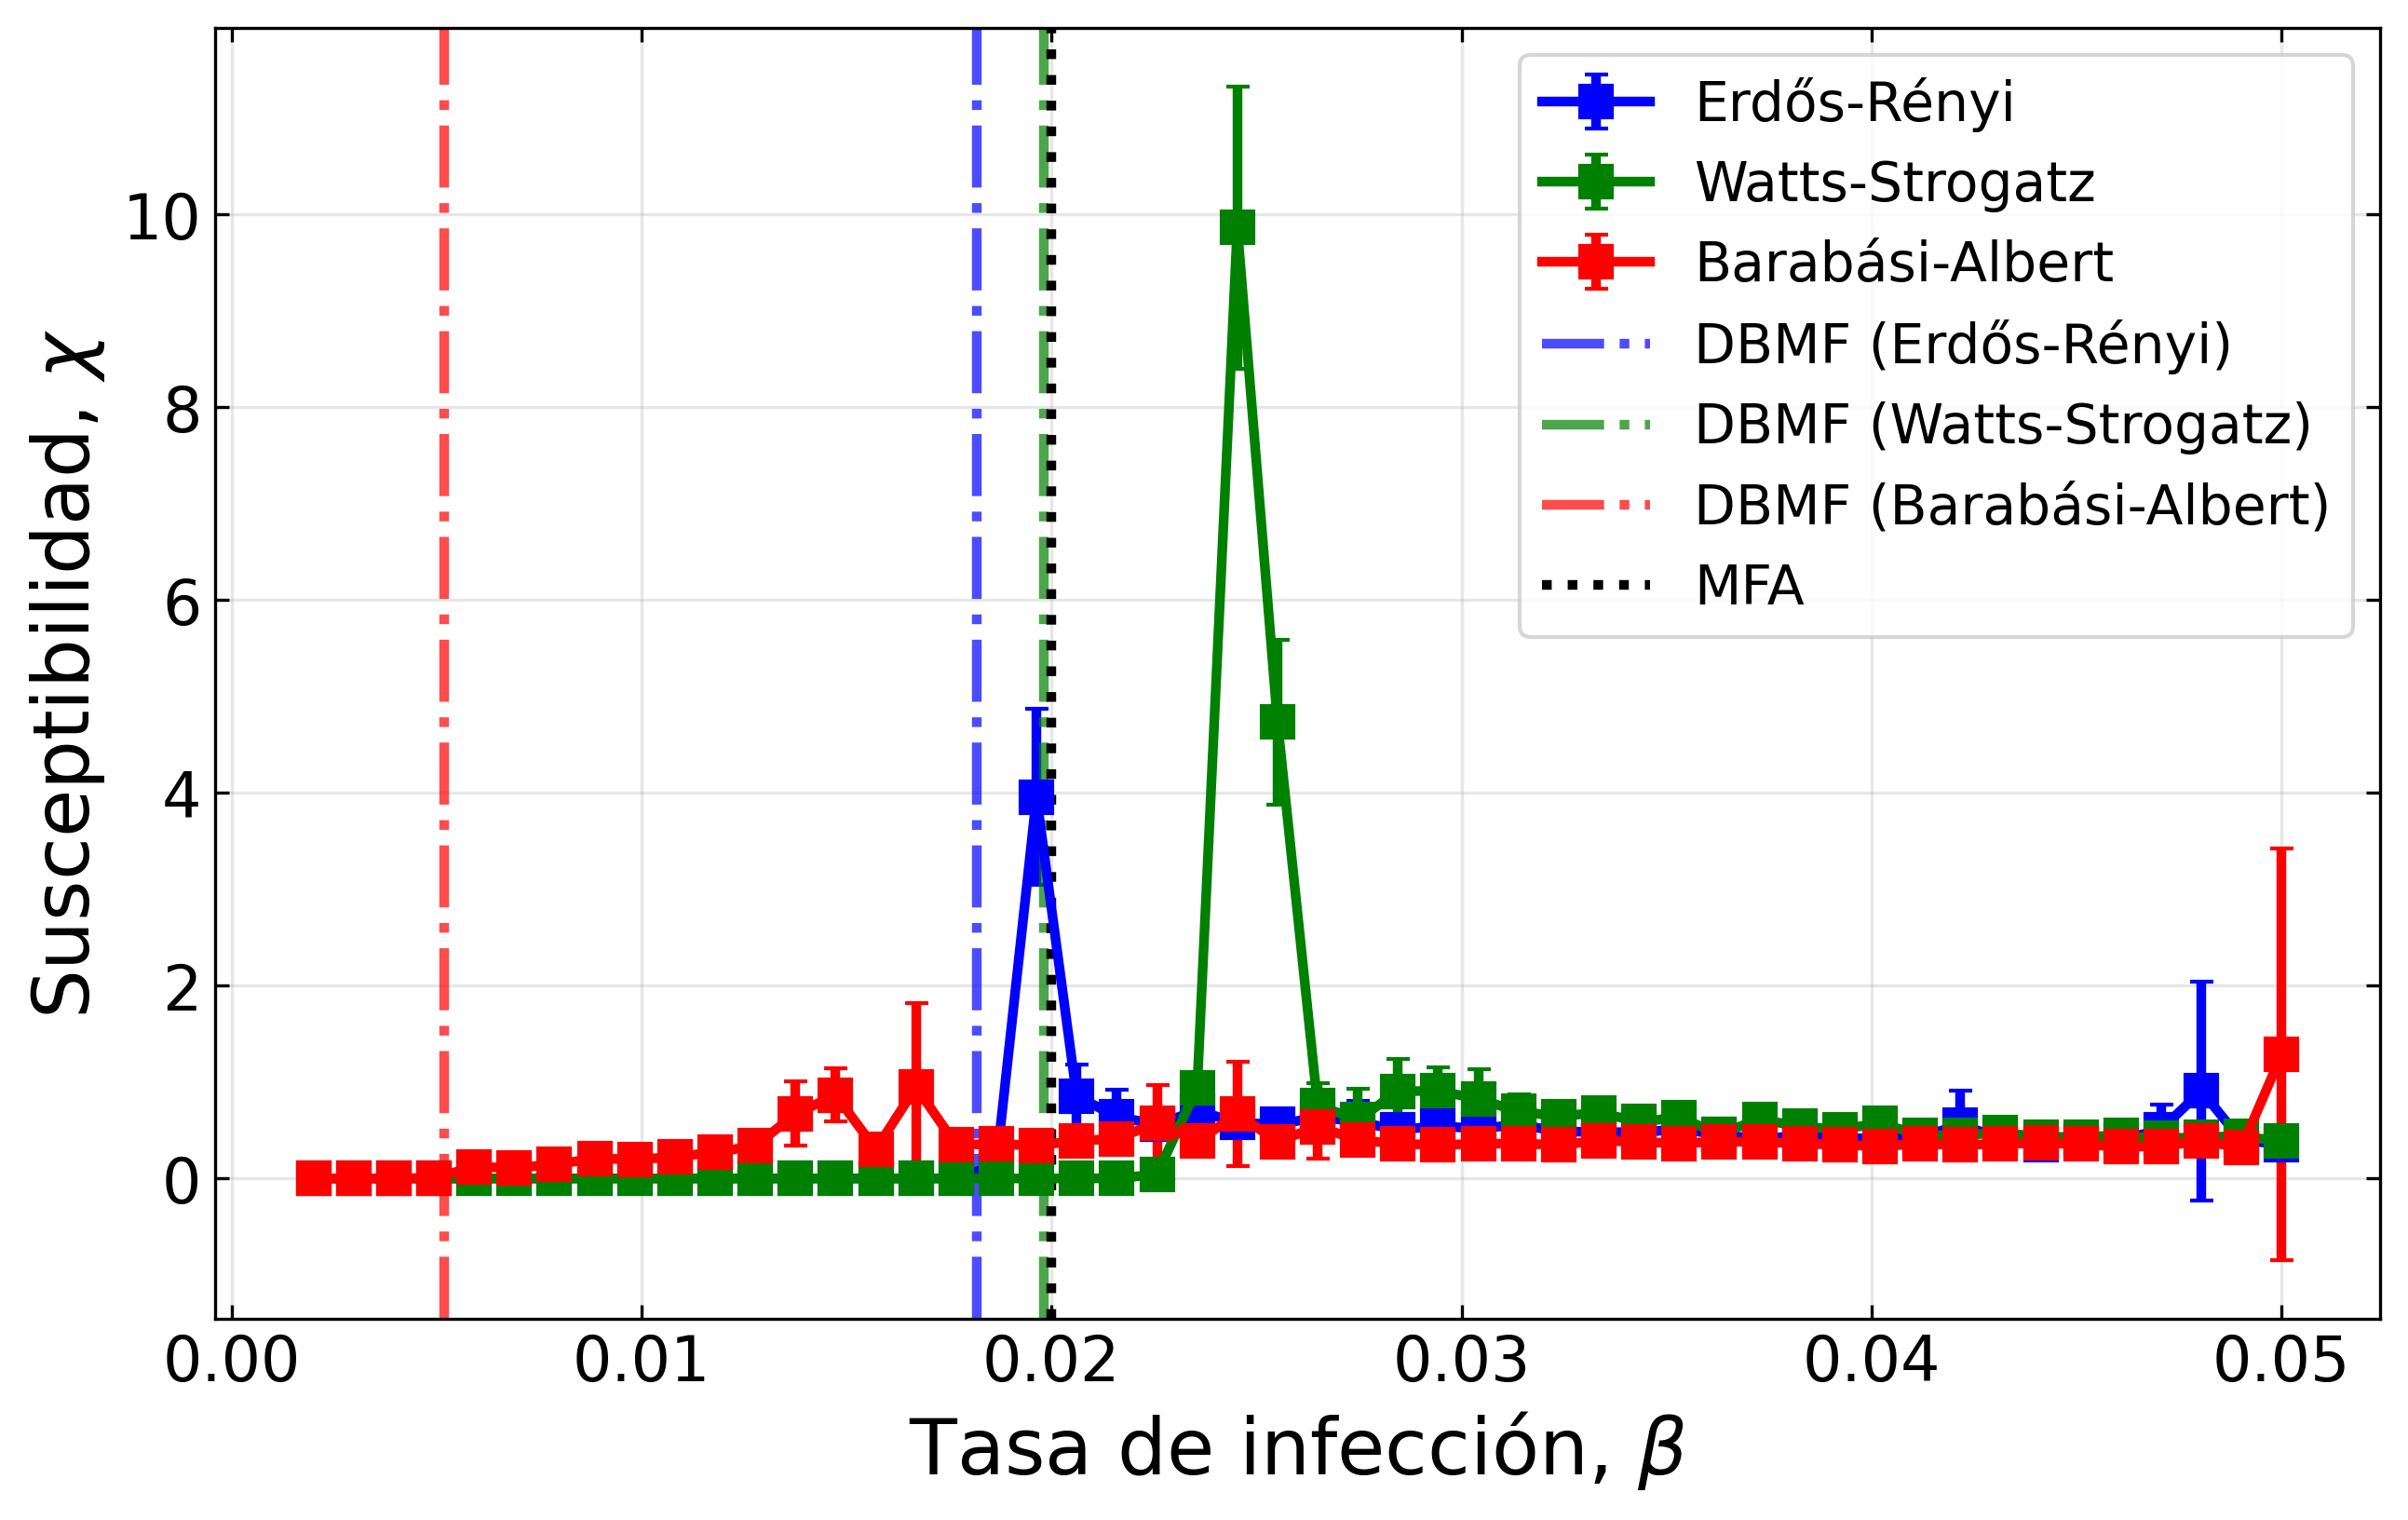
\includegraphics[width=\columnwidth]{imagenes/6_comparison_susceptibility_N500000.png}
		\caption{Susceptibilidad $\chi$ frente a la tasa de infección. Las transiciones en las redes ER y WS están marcadas por picos agudos, mientras que la red BA muestra un comportamiento degenerado.}
		\label{fig:susc}
	\end{figure}
	
	El comportamiento de la red de Barabási-Albert resulta particularmente relevante debido a su estructura de red libre de escala. A diferencia de las topologías homogéneas, donde la transición ocurre a un valor de $\beta$ bien definido, la presencia de \textit{superhubs} de grado extremadamente alto en la red BA propicia que la epidemia sea capaz de persistir incluso bajo tasas de infección infinitesimales. Esta característica topológica se manifiesta en una supresión del umbral epidémico que se evidencia claramente al realizar un análisis de detalle en la proximidad del origen. Esto se observa en la Figura \ref{fig:ba_zoom}.
	
	% --- BLOQUE DE OPCIONES PARA LA GRÁFICA DE BARABÁSI-ALBERT ---
	% Descomenta solo la opción que prefieras para mostrar el detalle del colapso del umbral.
	
	% OPCIÓN 1: Solo el zoom independiente
	% \begin{figure}[htbp]
		%     \centering
		%     \includegraphics[width=\columnwidth]{1_Barabasi_Albert_phase_transition_ZOOM_ONLY.png}
		%     \caption{Detalle de la transición de fase en la red de Barabási-Albert para bajas tasas de infección, ilustrando cómo el aumento del tamaño de la red $N$ desplaza el umbral hacia el origen.}
		%     \label{fig:ba_zoom}
		% \end{figure}
	
	% OPCIÓN 2: Gráfica principal con el inset anidado (RECOMENDADO PARA AHORRAR ESPACIO)
	\begin{figure}[htbp]
		\centering
		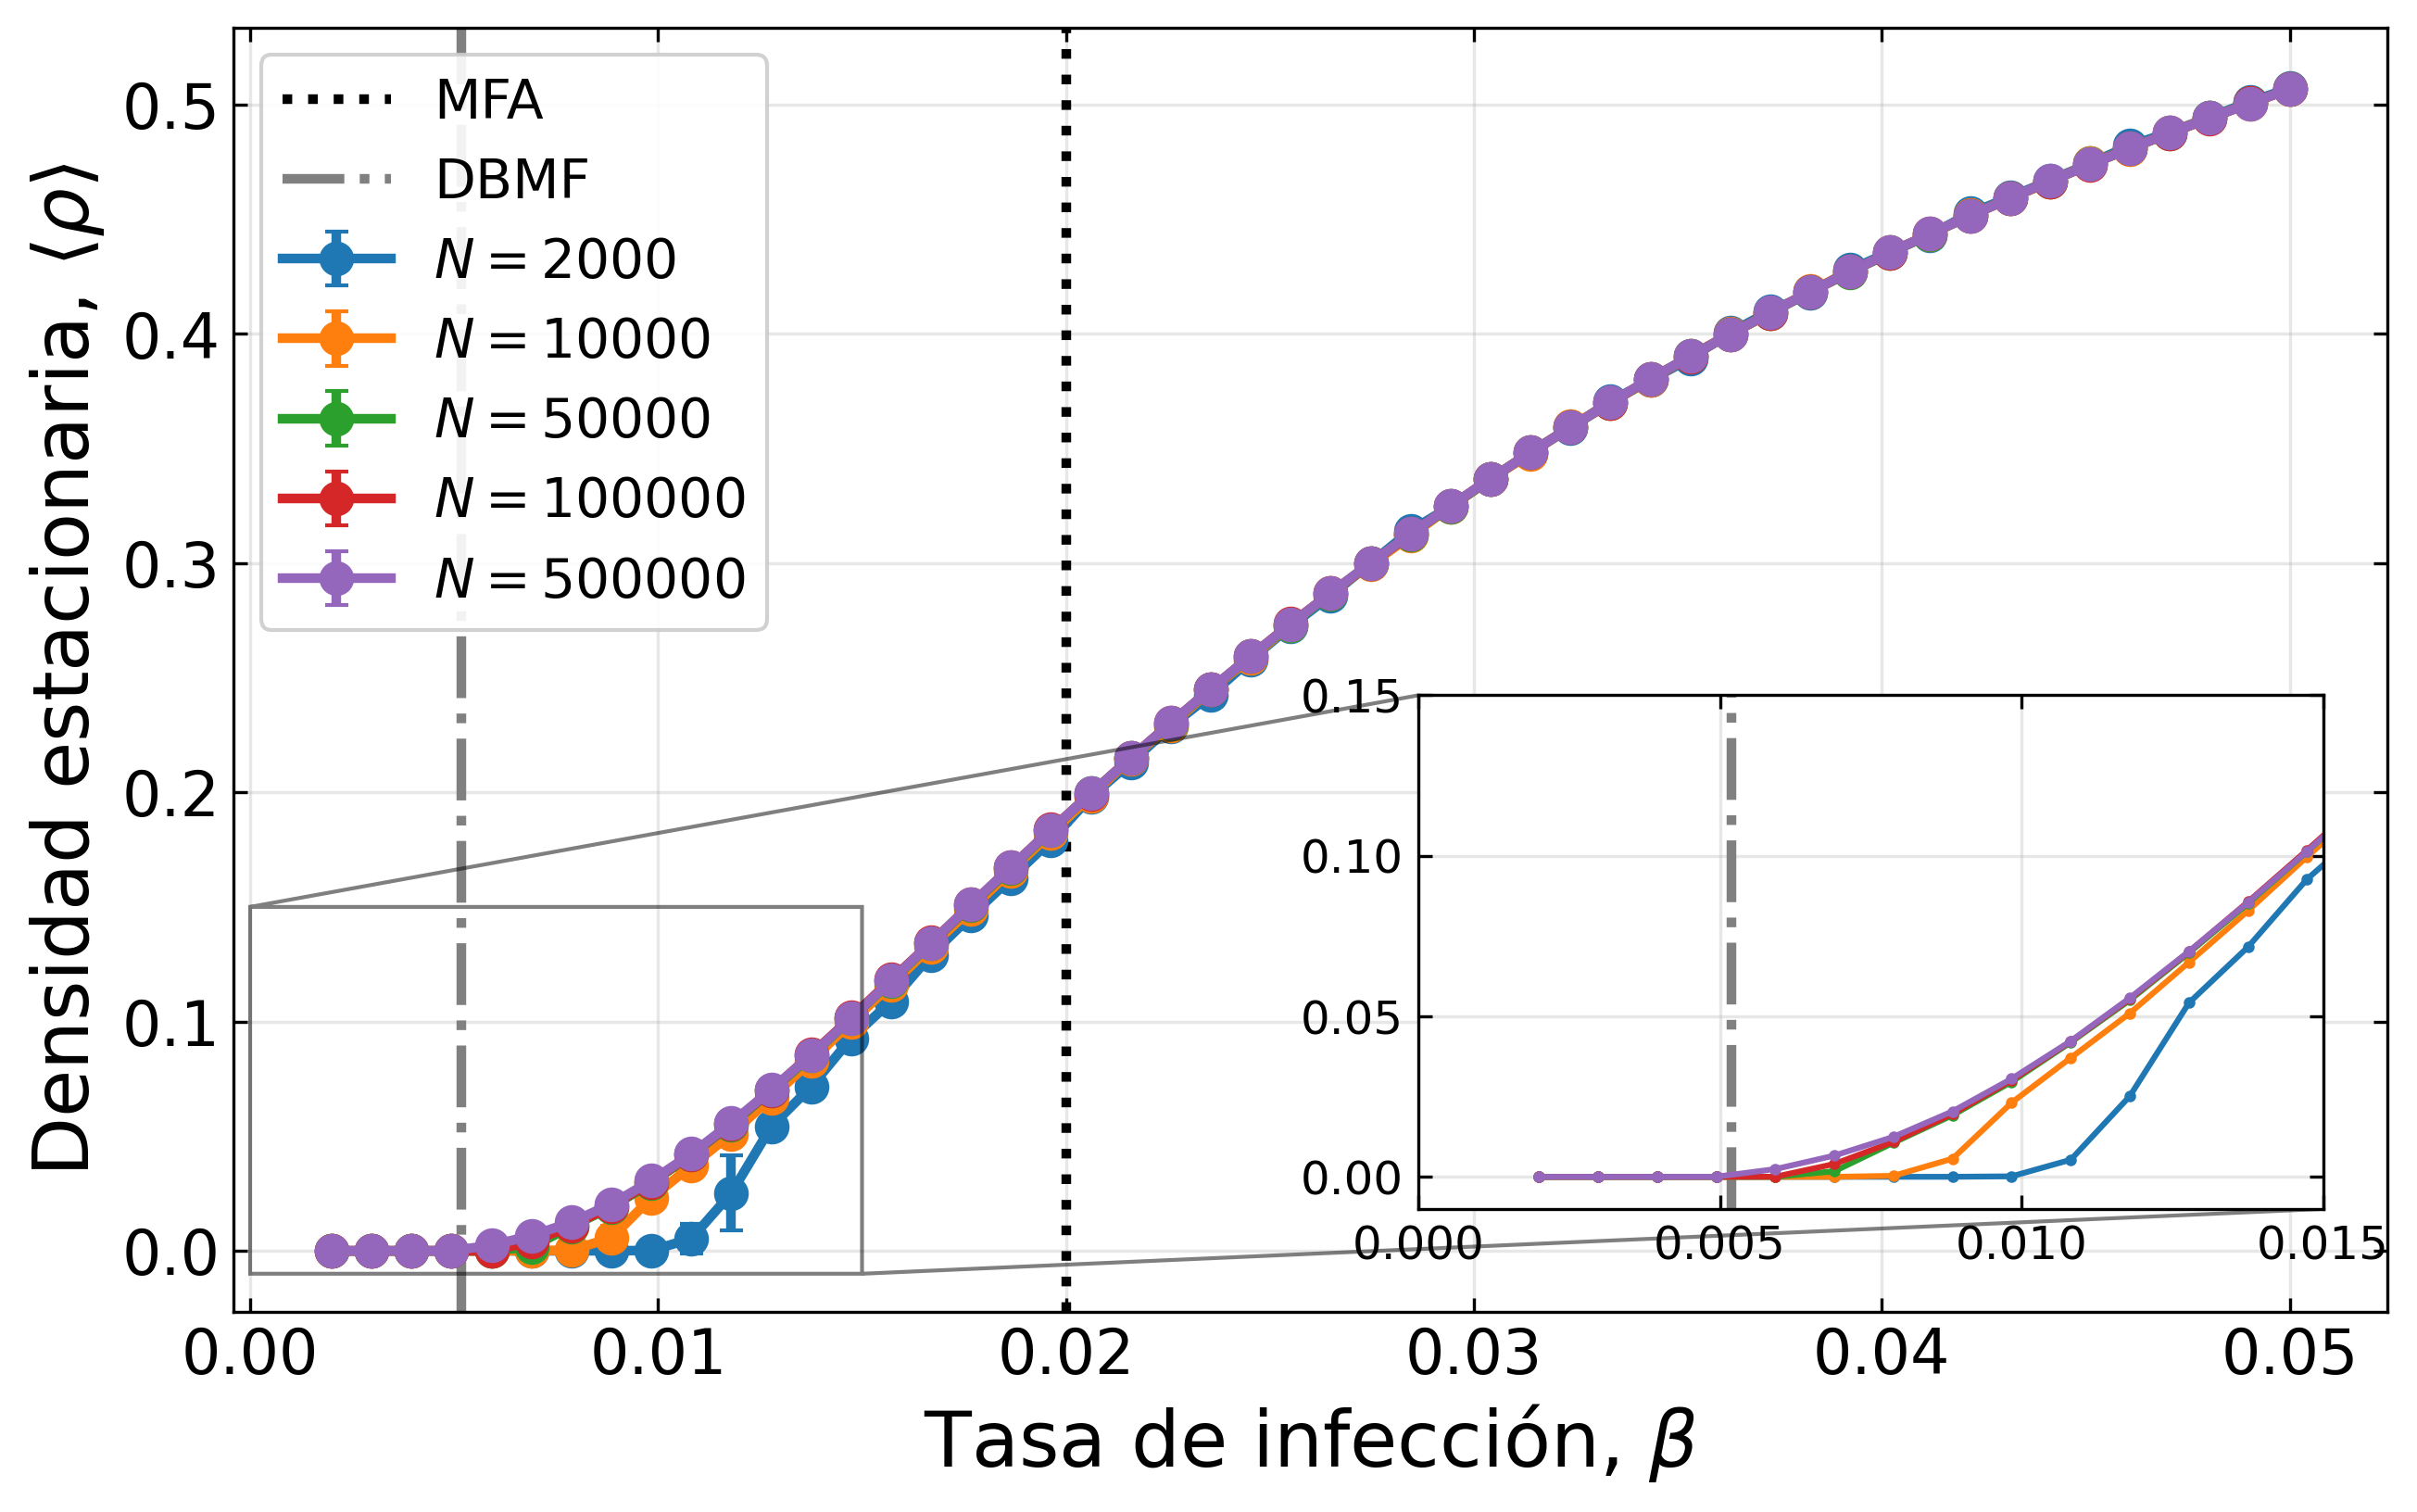
\includegraphics[width=\columnwidth]{imagenes/1_Barabasi_Albert_phase_transition_WITH_INSET.png}
		\caption{Transición de fase en la red de Barabási-Albert. El recuadro interior (inset) detalla la región cercana al origen, mostrando los efectos de tamaño finito y el colapso del umbral epidémico a medida que $N \to \infty$.}
		\label{fig:ba_zoom}
	\end{figure}
	% -----------------------------------------------------------
	
	\subsection{Escalamiento y Clases de Universalidad}
	\label{subsec:esc_uni}
	Cerca del umbral crítico, la teoría de fenómenos críticos predice que el parámetro de orden obedece una ley de potencias del tipo:
	\begin{equation}
		\rho \sim (\beta - \beta_c)^\alpha
	\end{equation}
	\textit{Nota: Por claridad notacional, se empleará el exponente $\alpha$ en lugar del tradicional $\beta$ de la literatura estadística, evitando así confusión con la tasa de infección macroscópica del modelo SIS.}
	
	Al representar los datos en escala logarítmica (Fig. \ref{fig:scaling}), el exponente $\alpha$ corresponde a la pendiente de la recta en la región asintótica. Los resultados numéricos revelan pendientes casi idénticas para las topologías ER ($\alpha \approx 0.91$) y WS ($\alpha \approx 0.97$), ubicándolas dentro de la clase de universalidad de percolación dirigida en campo medio (véase el Apéndice \ref{apendice:percolacion_dirigida}), en la que se trabaja con un exponente estático teórico $\alpha=1$.
	
	Por el contrario, la red de Barabási-Albert ($\alpha \approx 0.03$) rompe de manera contundente con esta clase de universalidad, manifestando dinámicas anómalas intrínsecas a las redes con varianza de grado divergente.
	
	\begin{figure}[htbp]
		\centering
		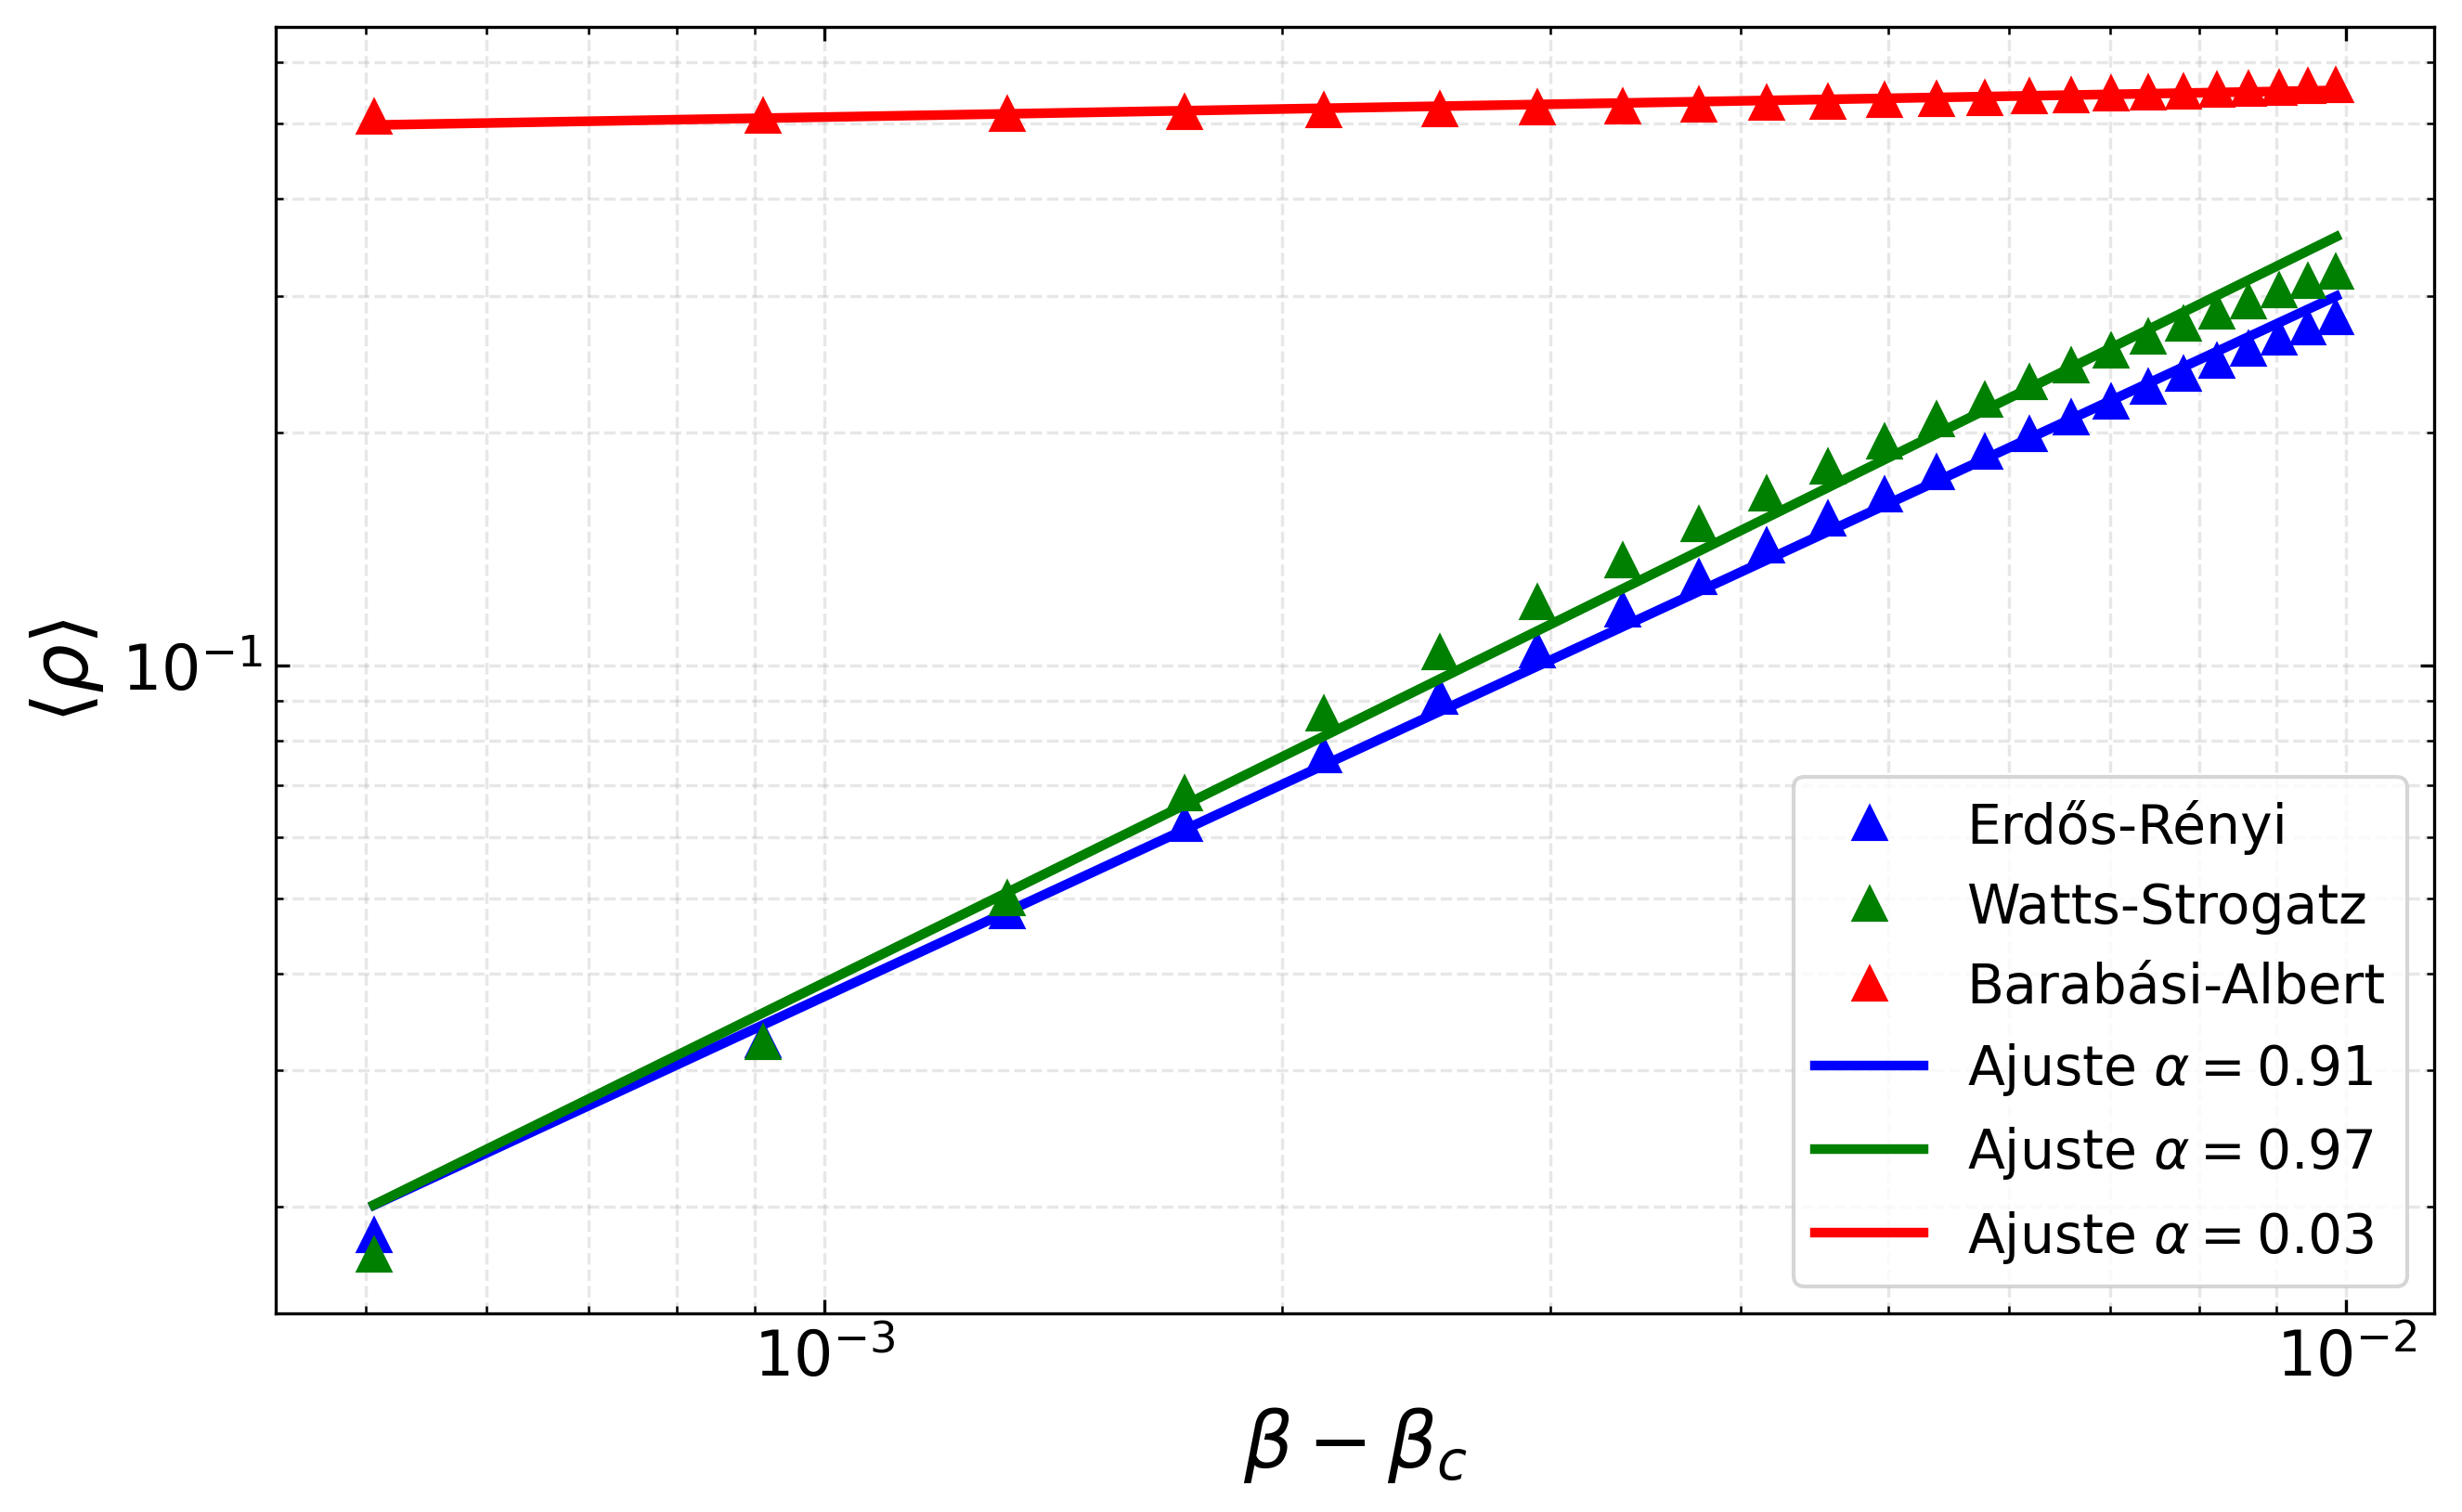
\includegraphics[width=\columnwidth]{imagenes/7_comparison_critical_scaling_N500000.png}
		\caption{Escalamiento crítico del modelo SIS. Las redes ER y WS comparten clase de universalidad, evidenciado por sus pendientes paralelas, mientras que BA muestra un exponente anómalo.}
		\label{fig:scaling}
	\end{figure}
	
	
	\section{Desorden Congelado y Fases de Griffiths}
	
	En las secciones anteriores, el estudio de las redes complejas se ha centrado en la heterogeneidad topológica, asumiendo que las tasas de infección y recuperación son homogéneas para todos los individuos de la población. Sin embargo, en epidemias reales, la heterogeneidad intrínseca de los nodos es ineludible debido a factores como variaciones en el sistema inmunológico, medidas de protección individual o, en el contexto de virus informáticos, la disparidad en los sistemas de seguridad.~\cite{PastorSatorras2015,Muñoz2010,Noest1986}
	
	Para modelar este fenómeno, se introduce el concepto de desorden congelado (\textit{quenched disorder}), en el cual la tasa de infección no es una constante global, sino una propiedad estática y heterogénea asignada a cada nodo $i$ al inicio de la simulación y que permanece invariable en el tiempo. Bajo ciertas condiciones estructurales, este desorden induce anomalías dinámicas macroscópicas dominadas por las fluctuaciones estadísticas de la red.~\cite{Muñoz2010,Noest1986,Odor2004}
	
	Incluso cuando el sistema se encuentra globalmente en la fase absorbente, la heterogeneidad estática permite la formación fortuita de \textit{regiones raras} o islas locales. Estas regiones están compuestas por clústeres de nodos con tasas de infección inusualmente altas o fuertemente conectados. La física fundamental de estas regiones raras dicta que la actividad epidémica confinada en su interior sobrevive durante periodos de tiempo extremadamente largos, los cuales crecen de forma exponencial respecto al tamaño físico de la isla.
	
	Aunque la infección en estas regiones raras ineludiblemente se acaba extinguiendo, la convolución matemática entre la probabilidad de existencia de una isla (que decae exponencialmente con su tamaño) y su tiempo de supervivencia (que crece exponencialmente) da como resultado una relajación macroscópica anómalamente lenta. La densidad total de infectados no decae de forma exponencial rápida, sino que sigue un decaimiento algebraico continuo dictado por una ley de potencias.
	
	A este régimen dinámico se le denomina Fase de Griffiths.~\cite{Noest1986,Muñoz2010,Odor2004} A diferencia del modelo SIS clásico, donde el decaimiento en forma de ley de potencias es un fenómeno estrictamente confinado al punto crítico y requiere un ajuste exacto de los parámetros (\textit{fine-tuning}), la Fase de Griffiths exhibe una invariancia de escala genérica. Es decir, el comportamiento algebraico se extiende sobre toda una región finita y extensa del espacio de parámetros, manifestándose como un espectro continuo de exponentes críticos variables.
	
	\subsection{Modelo Bimodal y Umbral de Percolación}
	
	Para estudiar sistemáticamente estos efectos en el modelo SIS, se adopta un modelo de desorden bimodal sobre redes aleatorias de Erdős-Rényi (ER).~\cite{Muñoz2010,PastorSatorras2015,Albert2002} La población se divide en dos clases: una fracción $1-q$ de nodos activos (tipo-I) con tasa de infección $\beta$, y una fracción $q$ de nodos inactivos (tipo-II) cuya tasa de infección se define como $r\beta$. En este trabajo, con el fin de maximizar el contraste dinámico y aislar topológicamente la propagación de la epidemia, se fija $r=0$, haciendo que los nodos tipo-II presenten una tasa de infección estrictamente nula.
	
	Mediante la aproximación de campo medio basada en el grado (DBMF), es posible derivar el umbral epidémico crítico para este sistema bimodal. Como se demuestra rigurosamente en el Apéndice \ref{apendice:bimodal_dbmf}, al particularizar la solución general para la topología estadística de una red de Erdős-Rényi, la tasa crítica de infección resultante obedece a la expresión:~\cite{Muñoz2010,PastorSatorras2015,Albert2002}
	\begin{equation}
		\beta_c^{DBMF}(q) = \mu \frac{1}{\langle k \rangle + 1} \frac{1}{1-q}
		\label{eq:beta_c_bimodal}
	\end{equation}
	Es fundamental notar que este resultado generaliza el umbral DBMF introducido en la sección anterior (Ec. \ref{eq:dbmf_threshold}). La introducción del desorden congelado modifica el umbral original ($\beta_c(0) = \mu \frac{\langle k \rangle}{\langle k^2 \rangle}$) escalándolo por un factor $(1-q)^{-1}$, evidenciando que la presencia de nodos inactivos incrementa la tasa de infección necesaria para sostener la epidemia de manera inversamente proporcional a la fracción activa de la red.
	
	Sin embargo, la propagación de la epidemia está supeditada a una transición puramente topológica: la percolación de sitios. Al silenciar una fracción $q$ de nodos, la topología efectiva disponible para el patógeno se reduce a una subred activa. Para que exista una componente gigante conexa de nodos tipo-I capaz de sostener una epidemia global, el grado medio de esta subred debe ser estrictamente mayor que la unidad. Como se detalla en el Apéndice \ref{apendice:percolacion}, esta condición estructural impone un umbral de fragmentación geométrico en la red dado por:
	\begin{equation}
		q_{perc} = 1 - \frac{1}{\langle k \rangle}
		\label{ec:q_perc}
	\end{equation}
	
	Si $q > q_{perc}$, la subred activa se fragmenta en clústeres finitos aislados, lo cual impide la propagación global del patógeno y confina la actividad epidémica a islas locales, sentando así las bases topológicas para la emergencia de los efectos de regiones raras. Para el estudio numérico posterior, se ha fijado una conectividad media $\langle k \rangle = 3$ y una tasa de recuperación $\mu = 0.3$, lo que define un umbral de percolación $q_{perc} = 2/3$. Las fronteras teóricas resultantes conforman el diagrama de fases ilustrado en la Fig. \ref{fig:diagrama_fases}.
	
	\begin{figure}[htbp]
		\centering
		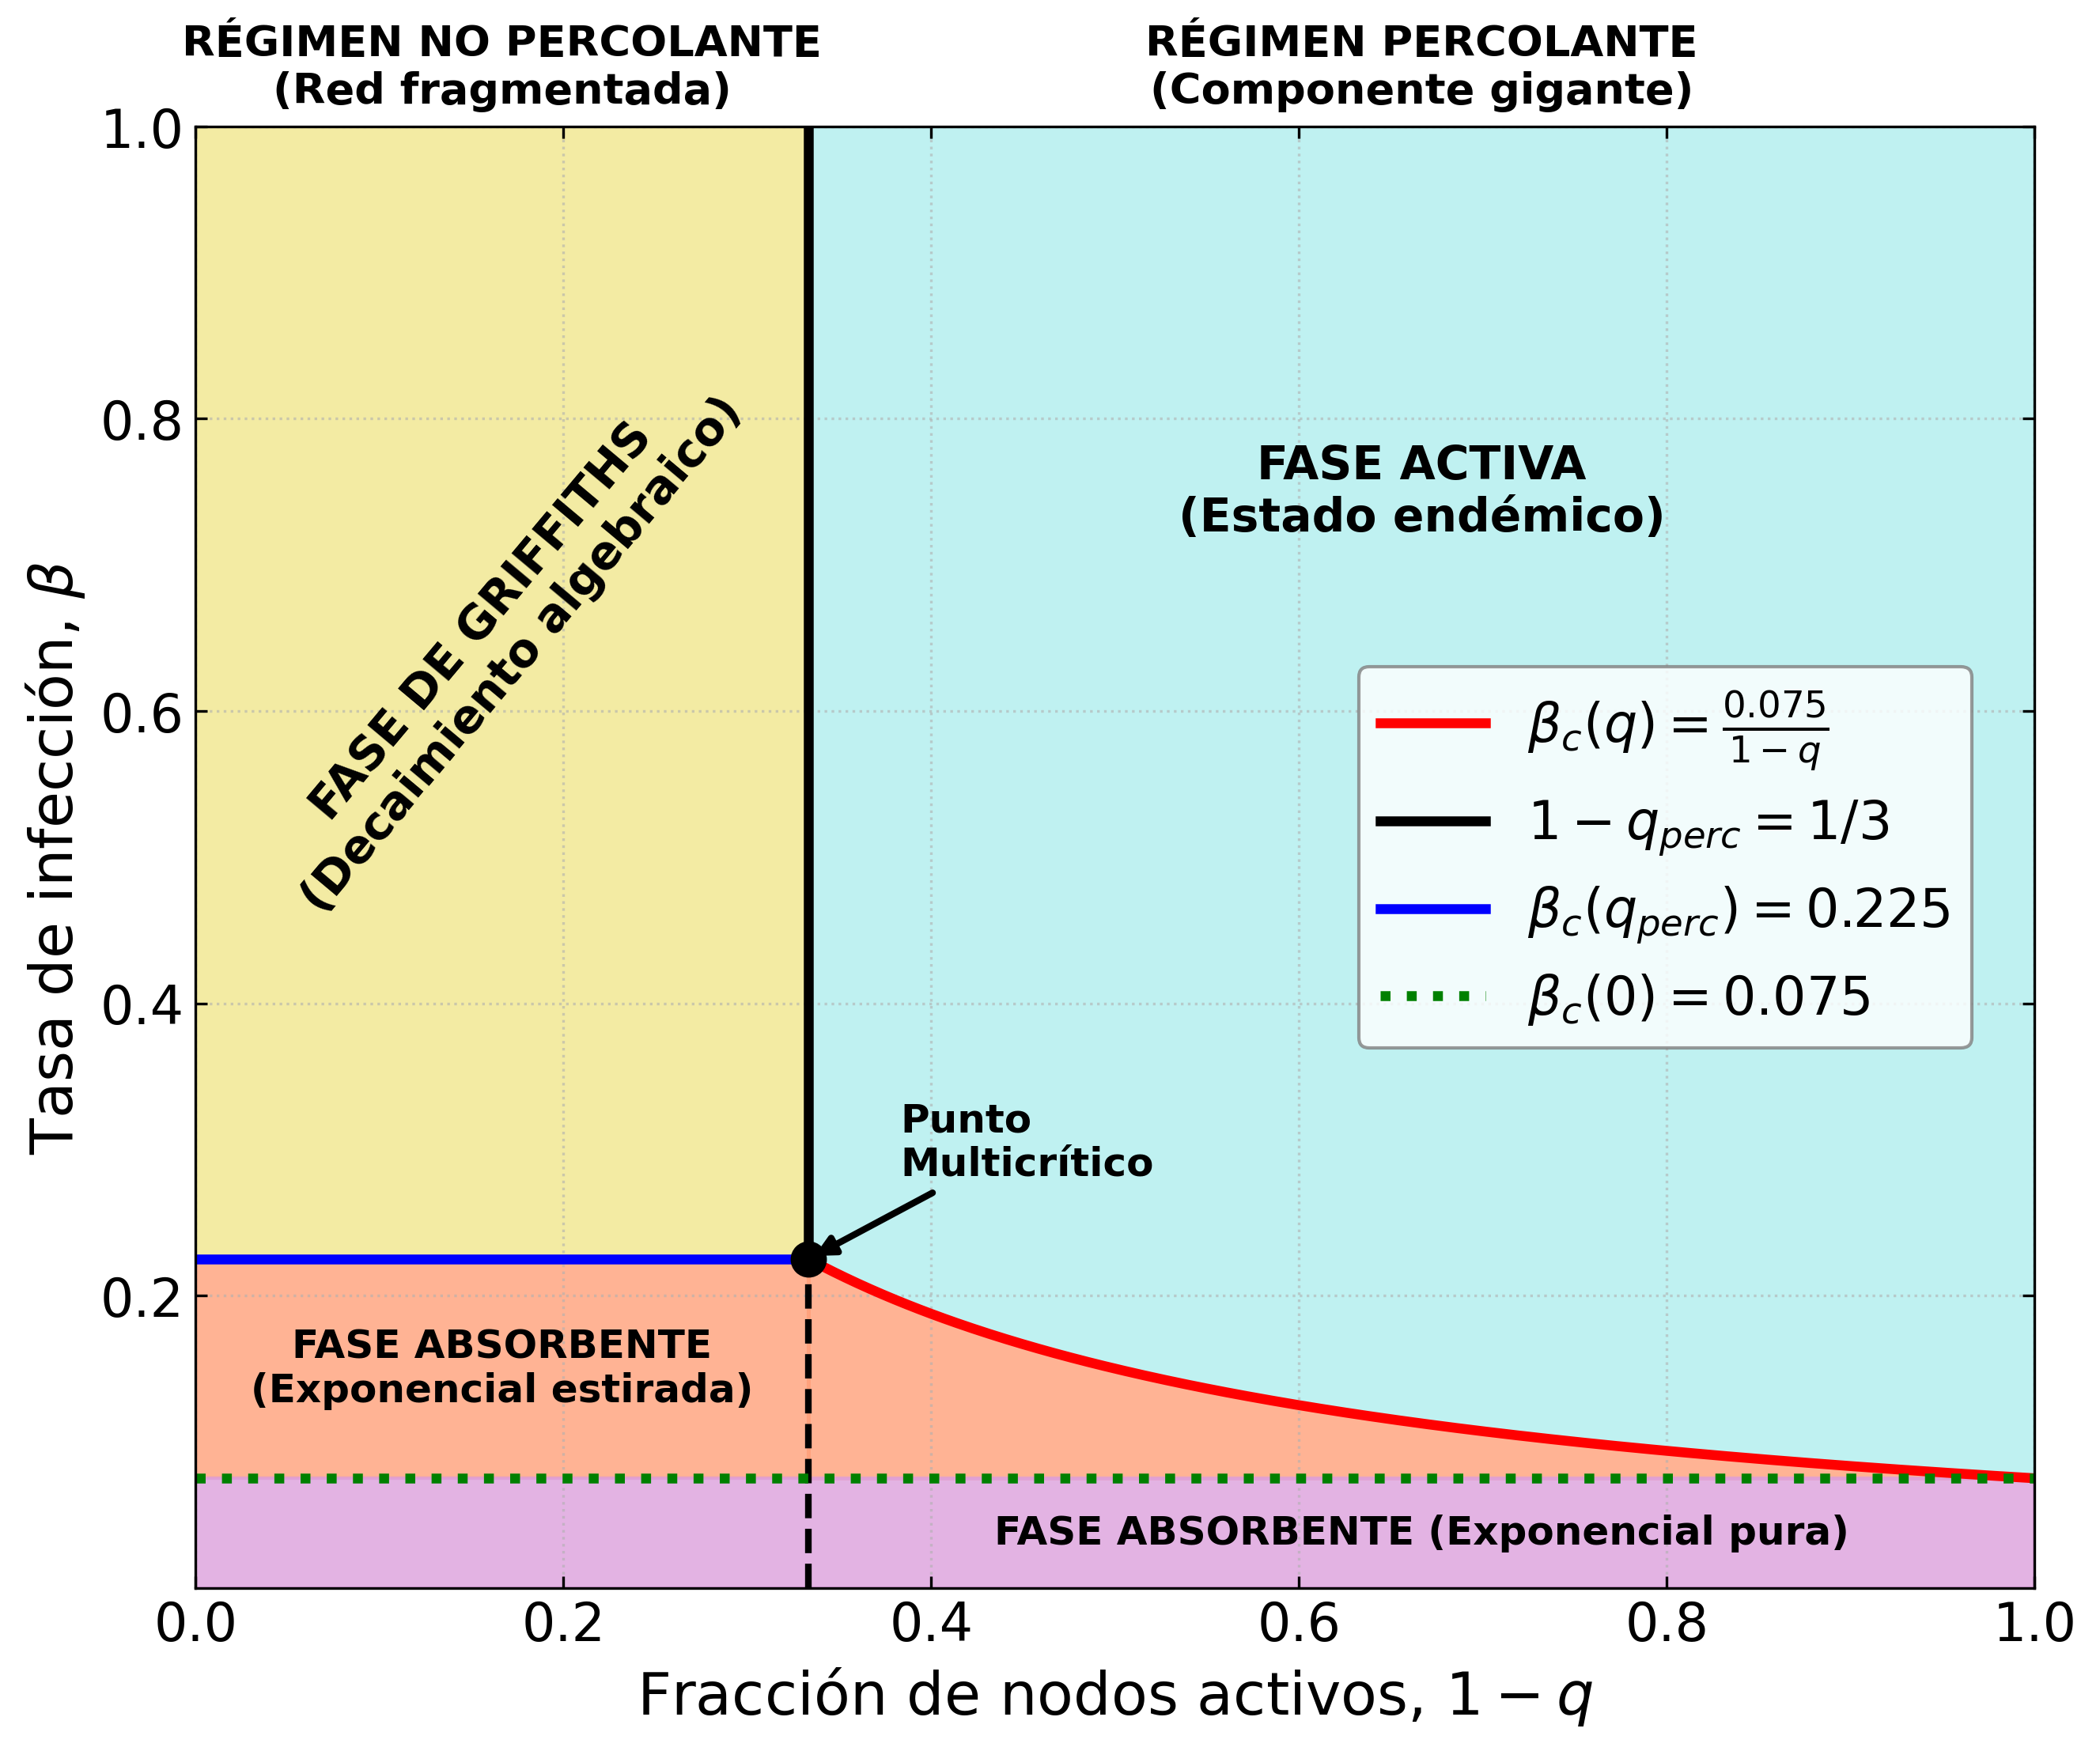
\includegraphics[width=\columnwidth]{imagenes/theoretical_phase_diagram_legend_formulas_only.png}
		\caption{Diagrama de fases teórico DBMF para el modelo SIS con desorden bimodal ($\langle k \rangle = 3$, $\mu=0.3$). La línea negra continua marca el umbral de percolación $q_{perc}=2/3$, dividiendo el sistema en un régimen de componente gigante y un régimen fragmentado.}
		\label{fig:diagrama_fases}
	\end{figure}
	
	Como se observa en el diagrama, el espacio de parámetros queda dividido estructuralmente por el umbral de percolación (línea negra discontinua y sólida vertical) situado en la fracción de nodos activos $1 - q_{perc} = 1/3$.~\cite{Albert2002,Dorogovtsev2008} A la derecha de esta frontera geométrica ($q < 2/3$), la red preserva su componente gigante, lo que permite la existencia de una Fase Activa (estado endémico) siempre que la tasa de infección $\beta$ supere la curva crítica teórica $\beta_c(q)$ dictada por la Ec. \ref{eq:beta_c_bimodal} (curva roja).
	
	Por el contrario, a la izquierda de la frontera ($q > 2/3$), el colapso topológico suprime por completo la posibilidad de un estado endémico global. En este régimen no percolante, la viabilidad temporal de la infección queda estratificada por dos límites teóricos constantes: el suelo crítico puro $\beta_c(0) = 0.075$, correspondiente al umbral de una red homogénea sin desorden ($q=0$), y el límite fragmentado $\beta_c(q_{perc}) = 0.225$, que marca la transición donde los clústeres aislados alcanzan localmente la criticidad. 
	
	La convergencia geométrica y dinámica de estas fronteras define un punto multicrítico en las coordenadas teóricas $(1/3, 0.225)$. Es precisamente en este sector fragmentado, delimitado numéricamente por los umbrales horizontales descritos, donde el sistema abandona el comportamiento binario clásico y despliega un espectro continuo de fases absorbentes.~\cite{Muñoz2010,Noest1986,Odor2004}
	
	\subsection{Dinámica de Relajación y Regímenes Anómalos}
	
	La fragmentación topológica descrita altera drásticamente la dinámica de relajación del sistema.~\cite{Muñoz2010,Noest1986,Odor2004} En el régimen fragmentado ($q > q_{perc}$), la densidad total de infectados $\rho(t)$ está gobernada por la Teoría de Fluctuaciones Óptimas, expresándose como la convolución estadística entre la probabilidad geométrica de hallar un clúster de tamaño $s$, dada por $\mathcal{P}(s)$, y el tiempo de supervivencia de la infección en dicho clúster, $\tau(s)$.
	
	El análisis asintótico de esta integral (desarrollado en detalle en el Apéndice \ref{apendice:fluctuaciones}) revela que la competición entre la estructura topológica~\cite{Muñoz2010,Noest1986,Odor2004} y el tiempo de supervivencia origina cuatro regímenes absorbentes fundamentales:
	\begin{itemize}
		\item \textbf{Fase de Griffiths:} Es el régimen más interesante. Para $\beta > \beta_c(q_{perc})$, el tiempo de vida en las islas activas crece exponencialmente, resultando en un decaimiento algebraico global $\rho(t) \sim t^{-\theta(q, \beta)}$. A medida que el sistema se aproxima a la fragmentación total ($q \to q_{perc}$), el exponente asintótico tiende a anularse ($\theta \to 0$), aplanando las curvas de decaimiento e indicando una transición continua.
		\item \textbf{Decaimiento Marginal:} Consecuencia directa del colapso del exponente $\theta$, exactamente en la frontera fractal de percolación ($q = q_{perc}$), la ley de potencias da paso a un decaimiento logarítmico, $\rho(t) \sim (\ln t)^{-1/2}$.
		\item \textbf{Exponencial Estirada:} Para $\beta_c(0) < \beta < \beta_c(q_{perc})$, las islas existen pero son dinámicamente subcríticas, generando una relajación de la forma $\rho(t) \sim e^{-B t^\alpha}$.
		\item \textbf{Exponencial Pura:} Para tasas extremadamente débiles $\beta < \beta_c(0)$, la infección decae antes de explorar las islas, recuperando el decaimiento exponencial clásico $\rho(t) \sim e^{-t/\tau_0}$.
	\end{itemize}
	
	\subsection{Resultados Computacionales}
	
	Para validar este marco teórico, se han ejecutado extensas simulaciones estocásticas de tiempo discreto en redes ER de $N=100\,000$ nodos, promediadas sobre múltiples configuraciones de desorden.
	
	En el régimen no fragmentado (Fig. \ref{fig:espectro_q03}, $q=0.3 < q_{perc}$), el sistema exhibe un comportamiento estándar de campo medio. Al superar la línea crítica $\beta_c(q)$, la densidad converge hacia un estado estacionario no nulo constante, confirmando la existencia de la fase activa endémica. Justo en la proximidad del umbral, la relajación obedece de manera precisa la ley de escala asintótica $\rho \sim t^{-1}$. Este decaimiento temporal, regido por un exponente dinámico unitario ($\delta = 1$), es totalmente coherente con el exponente estático del parámetro de orden ($\alpha \approx 1$) hallado en la sección \ref{subsec:esc_uni} y fundamentado analíticamente en el Apéndice \ref{apendice:percolacion_dirigida}, consolidando la pertenencia del sistema a la clase de universalidad de percolación dirigida en el límite de campo medio.
	
	\begin{figure}[htbp]
		\centering
		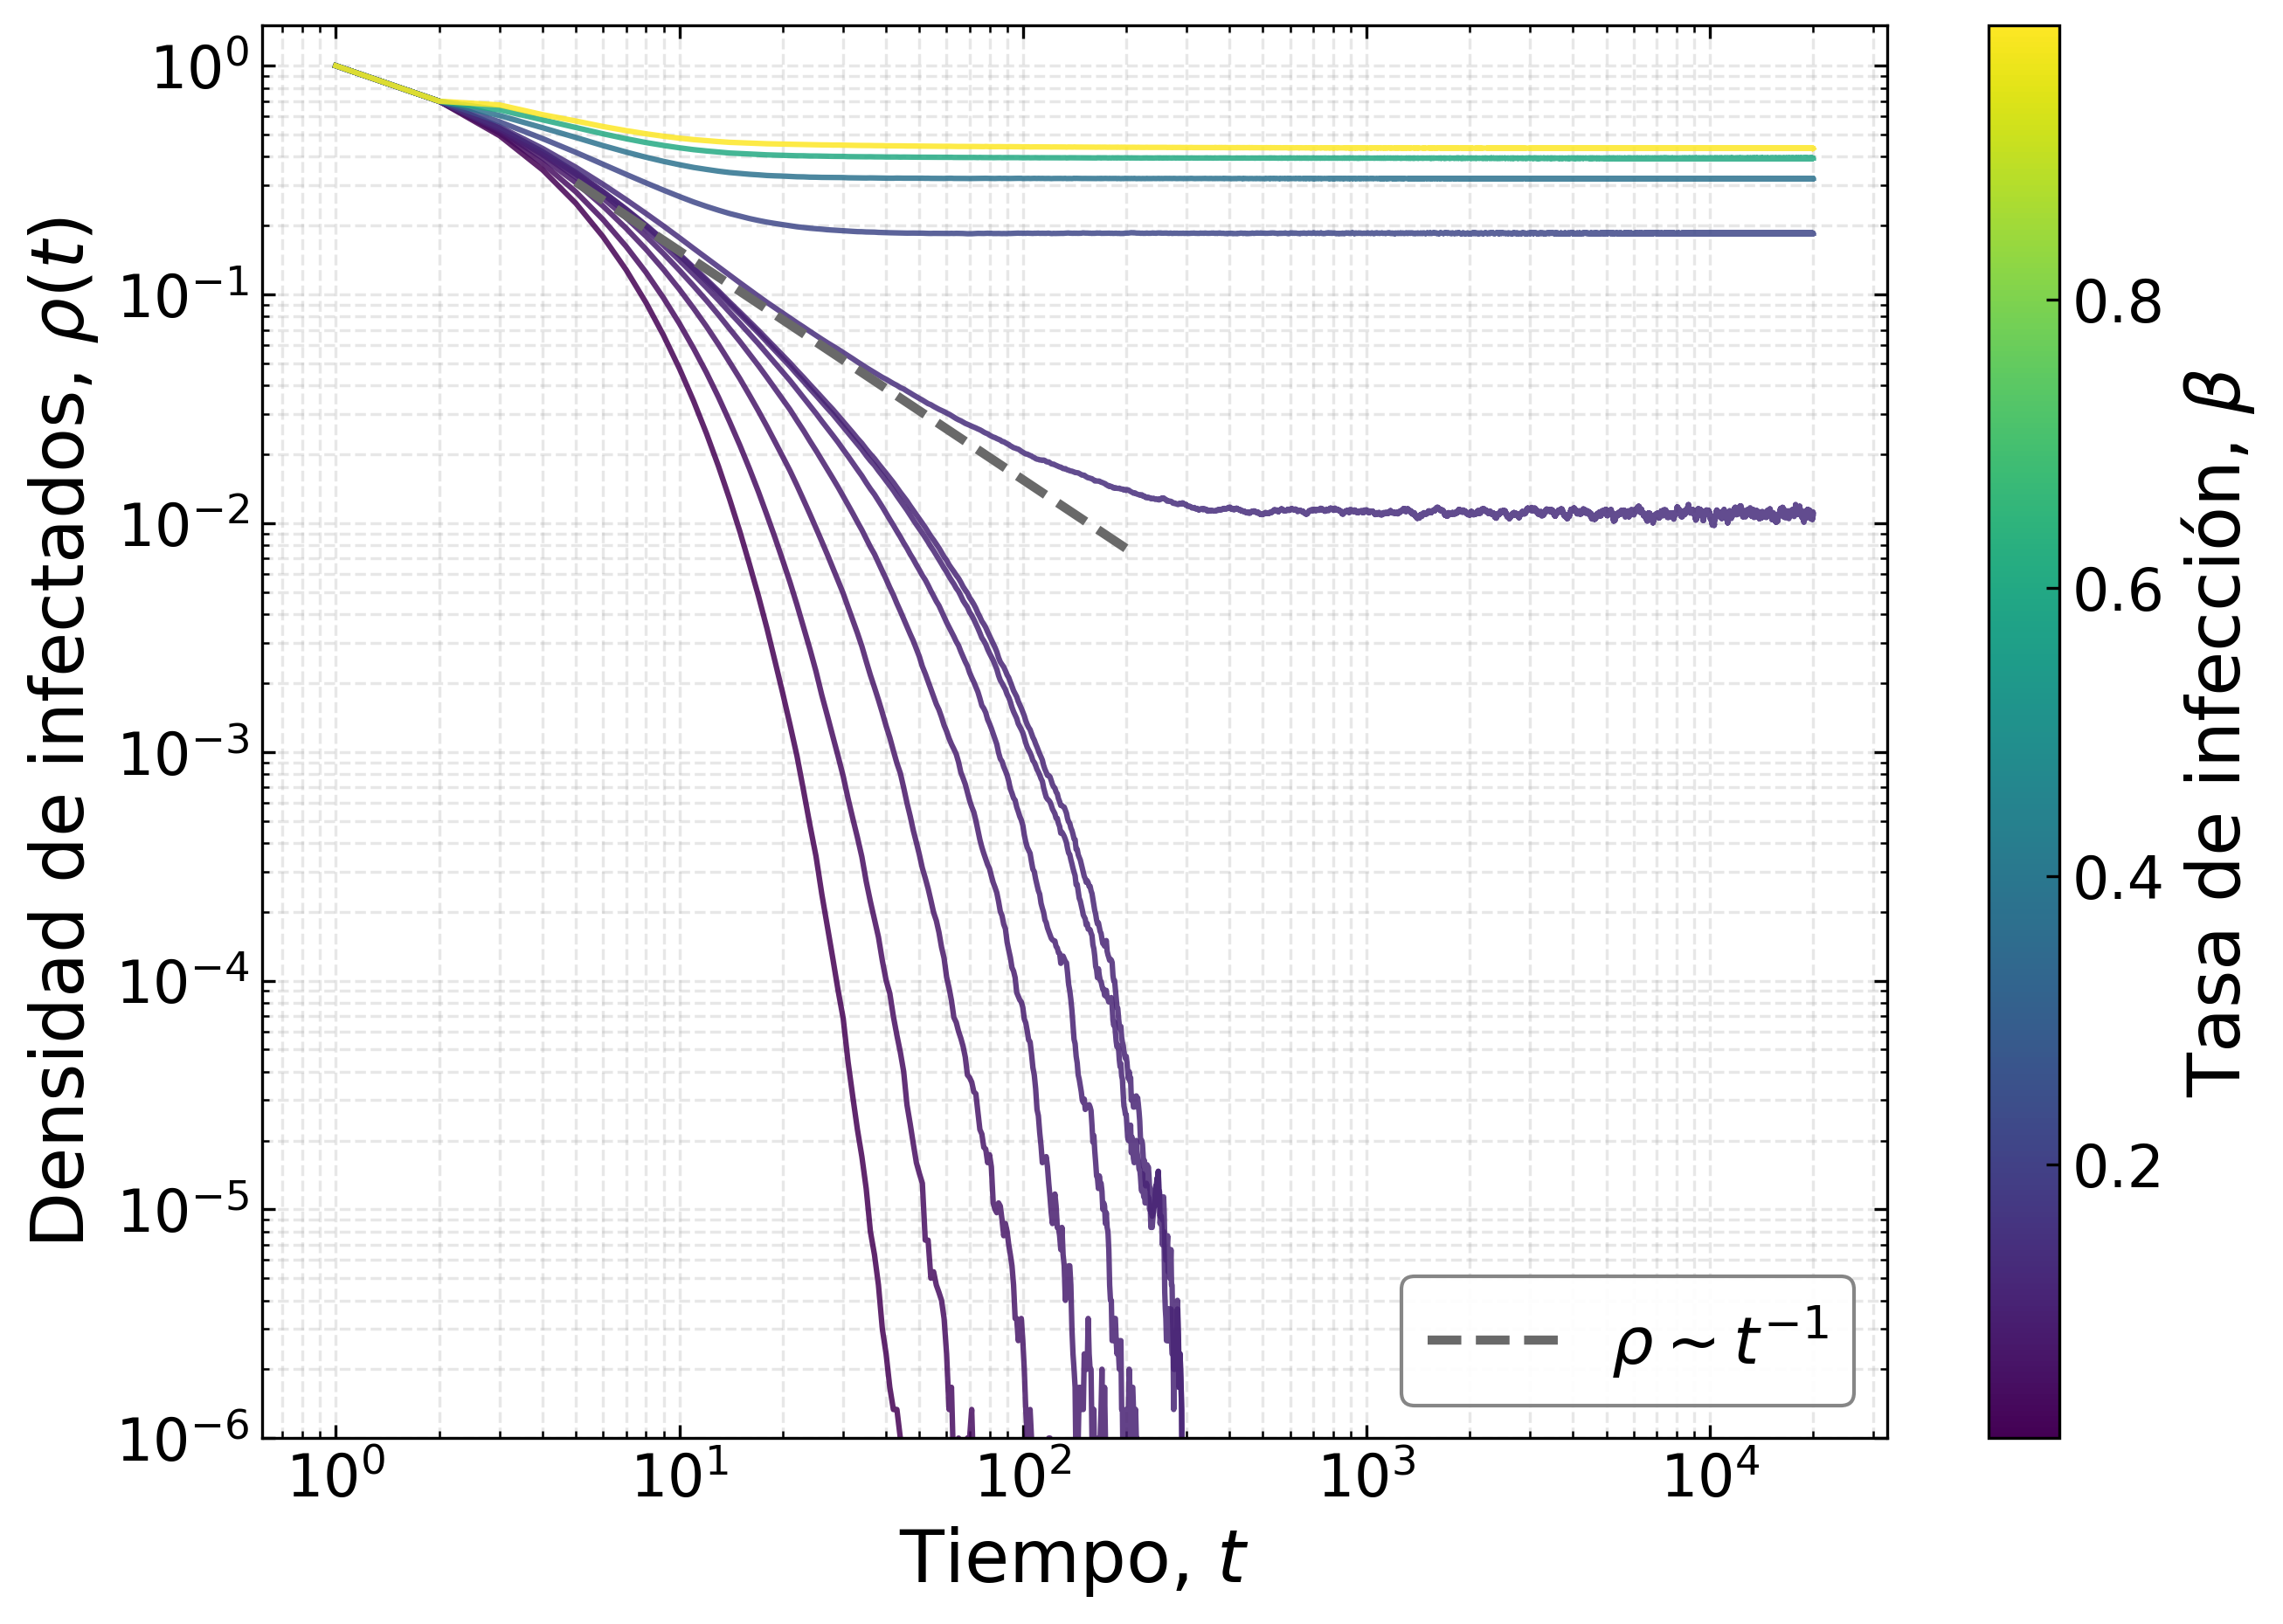
\includegraphics[width=0.9\columnwidth]{imagenes/summary_spectrum_q_0.30_selected.png}
		\caption{Densidad de infectados $\rho(t)$ para $q=0.30$ (Régimen percolante). Las curvas superan la línea crítica teórica y convergen hacia el estado endémico. La línea punteada indica el decaimiento crítico de campo medio esperado.}
		\label{fig:espectro_q03}
	\end{figure}
	
	Por el contrario, al inducir una fragmentación extrema ($q=0.9 > q_{perc}$), el estado endémico desaparece y el sistema decae hacia el estado absorbente. En esta región se observa un espectro continuo de regímenes de relajación. Para tasas de infección bajas, el parámetro de orden muestra caídas verticales abruptas en escala logarítmica, correspondientes a decaimientos exponenciales puros y estirados. A medida que se incrementa la tasa de infección, emerge un abanico de rectas con exponente algebraico dependiente del parámetro de control, característica definitoria de la Fase de Griffiths.
	
	Al contrastar las predicciones teóricas con los datos empíricos (Fig. \ref{fig:espectro_q09}), se observa una desviación sistemática en los umbrales de transición. Mientras que la aproximación DBMF establece el inicio analítico de la Fase de Griffiths en $\beta_c(q_{perc}) = 0.225$, las simulaciones revelan que el decaimiento algebraico estricto se manifiesta a valores superiores (e.g., $\beta \gtrsim 0.45$). Esta discrepancia es intrínseca a la naturaleza del modelo: las aproximaciones de campo medio asumen una mezcla topológica perfecta e ignoran las correlaciones dinámicas locales. En una red real, la reinfección mutua entre nodos vecinos favorece el estancamiento y la extinción prematura de la epidemia en los clústeres aislados. Al despreciar estas correlaciones, la aproximación DBMF sobreestima la capacidad de propagación, resultando en un umbral analítico estrictamente inferior al empírico.
	
	\begin{figure}[htbp]
		\centering
		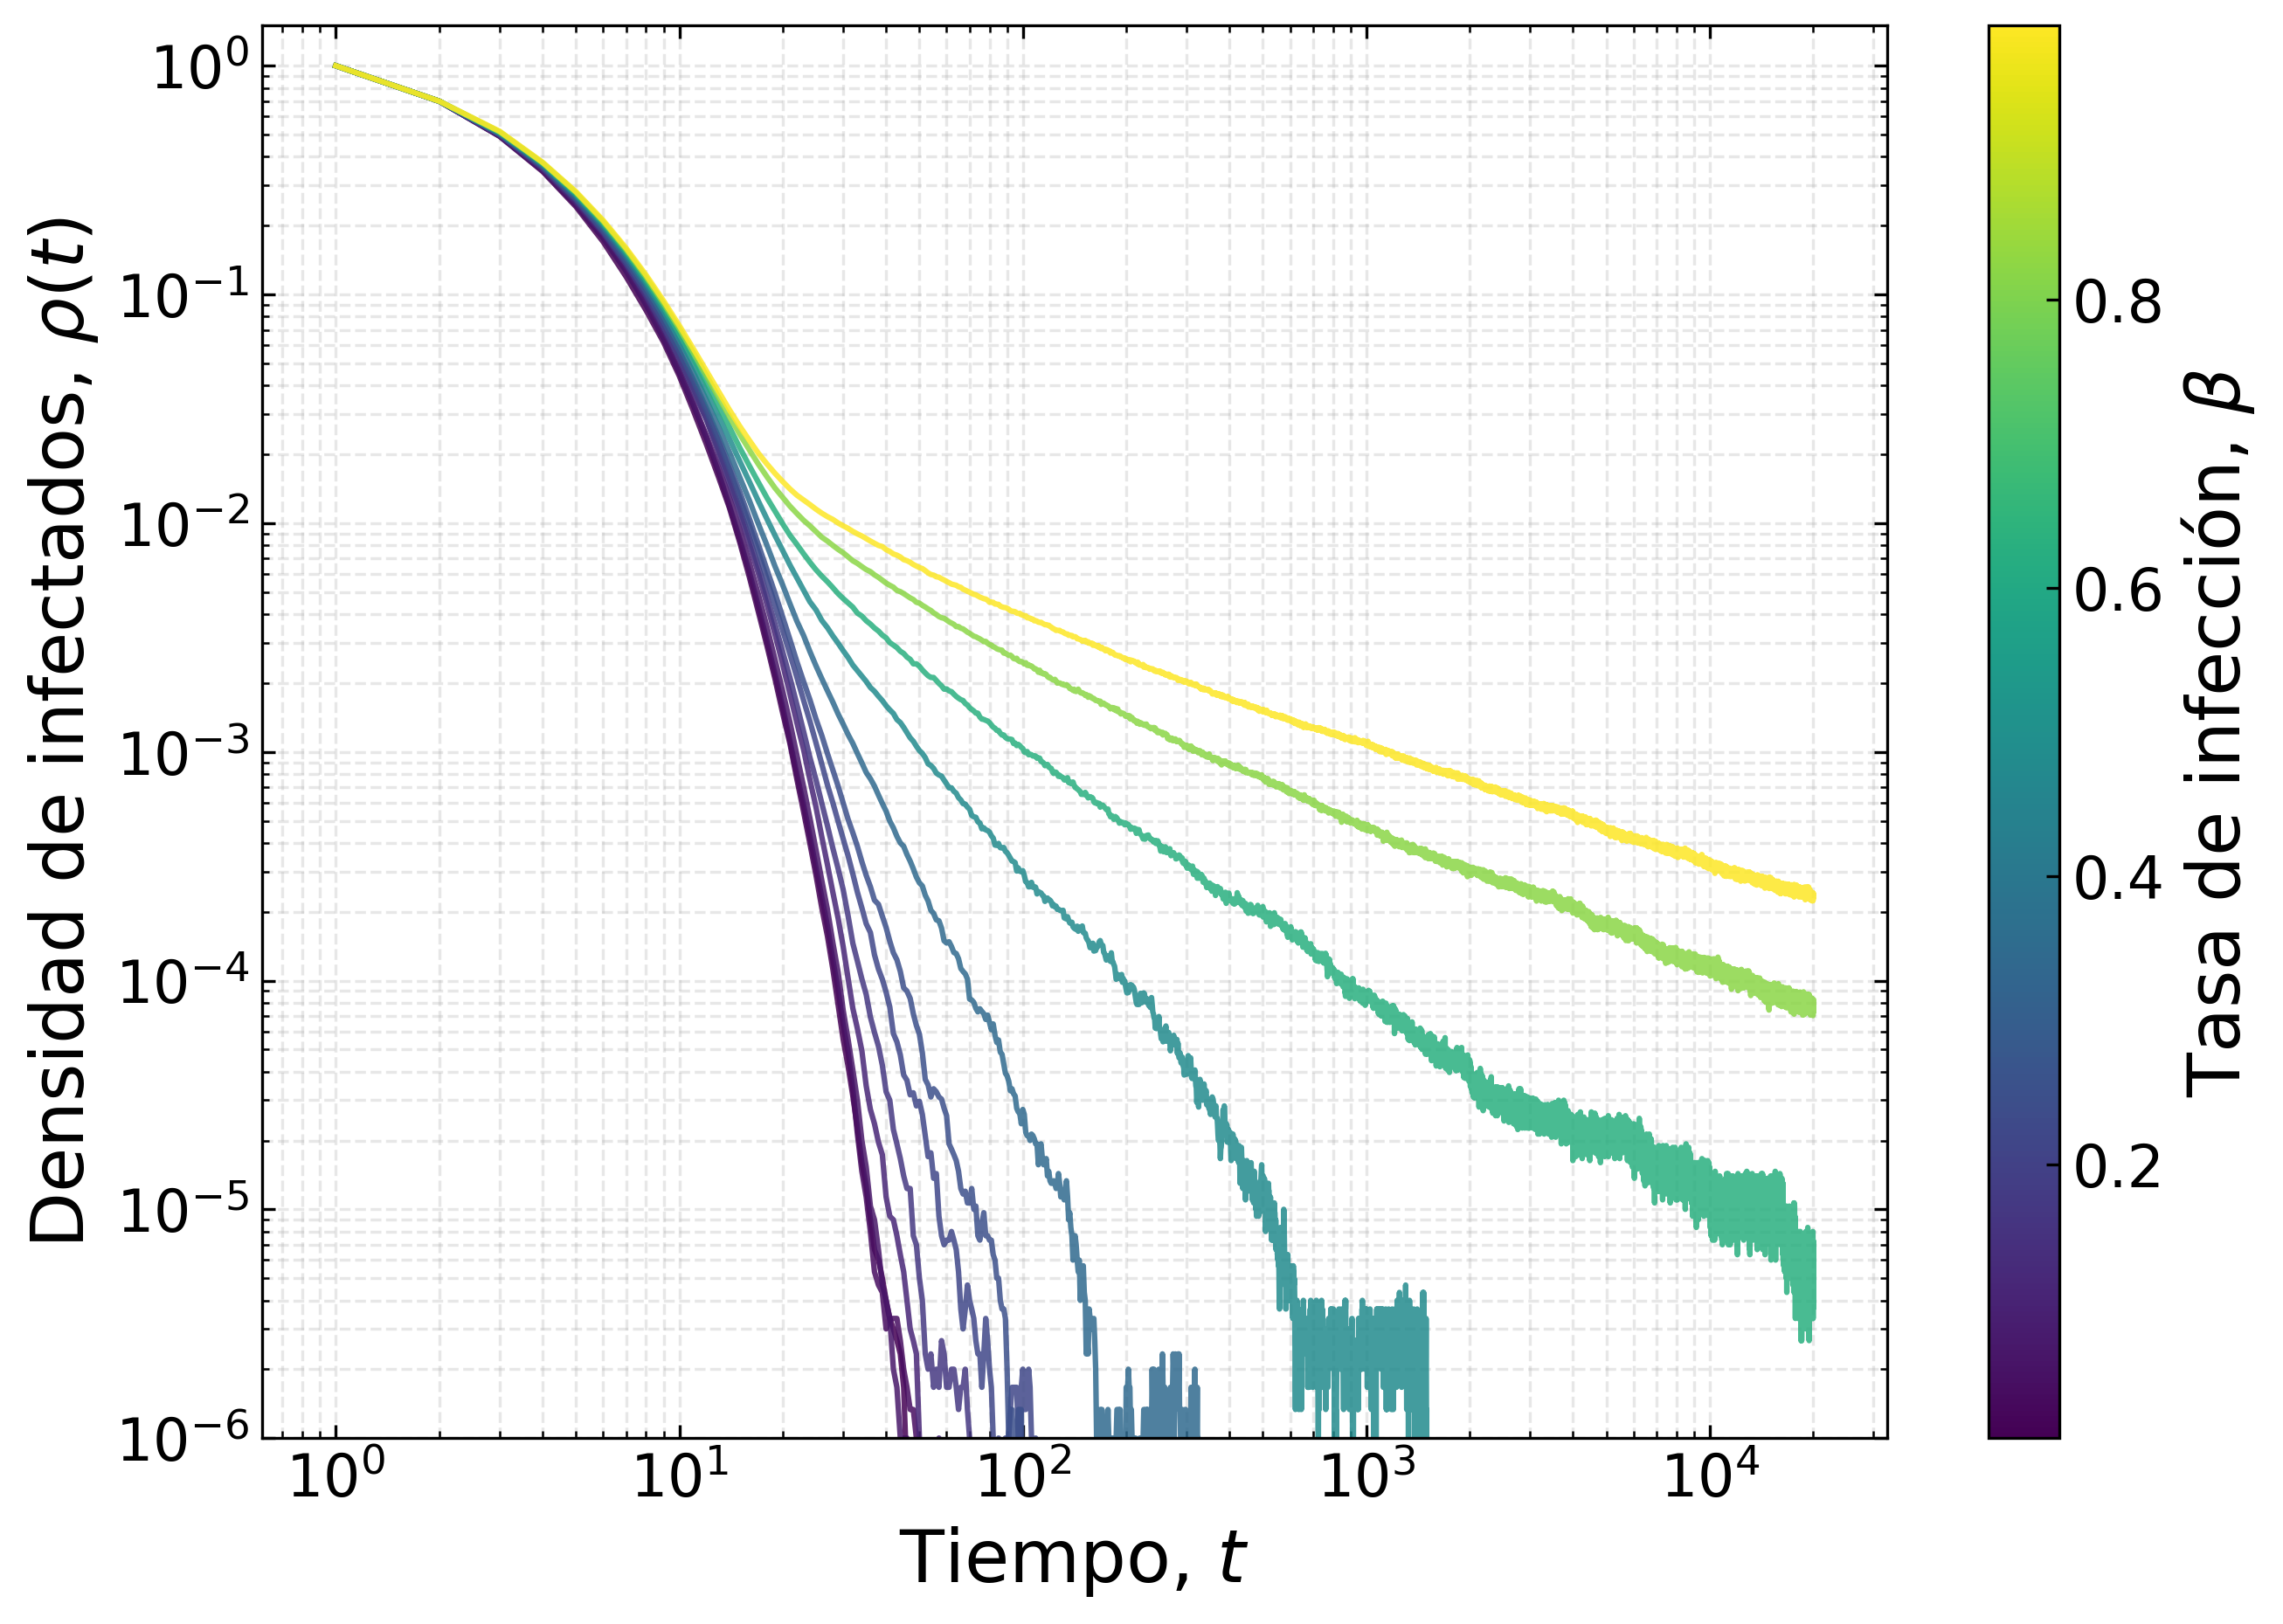
\includegraphics[width=0.9\columnwidth]{imagenes/summary_spectrum_q_0.90_selected.png}
		\caption{Espectro de relajación para $q=0.90$ (Régimen fragmentado). Se aprecia la transición continua desde decaimientos exponenciales rápidos hasta el comportamiento algebraico dependiente del parámetro propio de la Fase de Griffiths.}
		\label{fig:espectro_q09}
	\end{figure}
	
	En segundo lugar, el decaimiento algebraico asintótico predicho por la Teoría de Fluctuaciones Óptimas asume el límite termodinámico ($N \to \infty$), condición necesaria para permitir la existencia de regiones raras de tamaño arbitrariamente grande.~\cite{Muñoz2010,Noest1986,Odor2004} En simulaciones de tamaño finito ($N=10^5$), el tamaño estructural de dichas islas está matemáticamente acotado. En consecuencia, el tiempo máximo que el patógeno puede sobrevivir confinado en ellas está limitado, produciéndose un truncamiento por tamaño finito (\textit{finite-size cutoff}) que desvía la relajación algebraica hacia una caída exponencial. Como se evidencia en la Fig. \ref{fig:finite_size}, la duración del régimen invariante de escala crece sistemáticamente con el tamaño del sistema $N$, corroborando que la relajación anómala está dictada por las fluctuaciones de las regiones raras y su inevitable interrupción debido a la finitud física de la red.
	
	\begin{figure}[htbp]
		\centering
		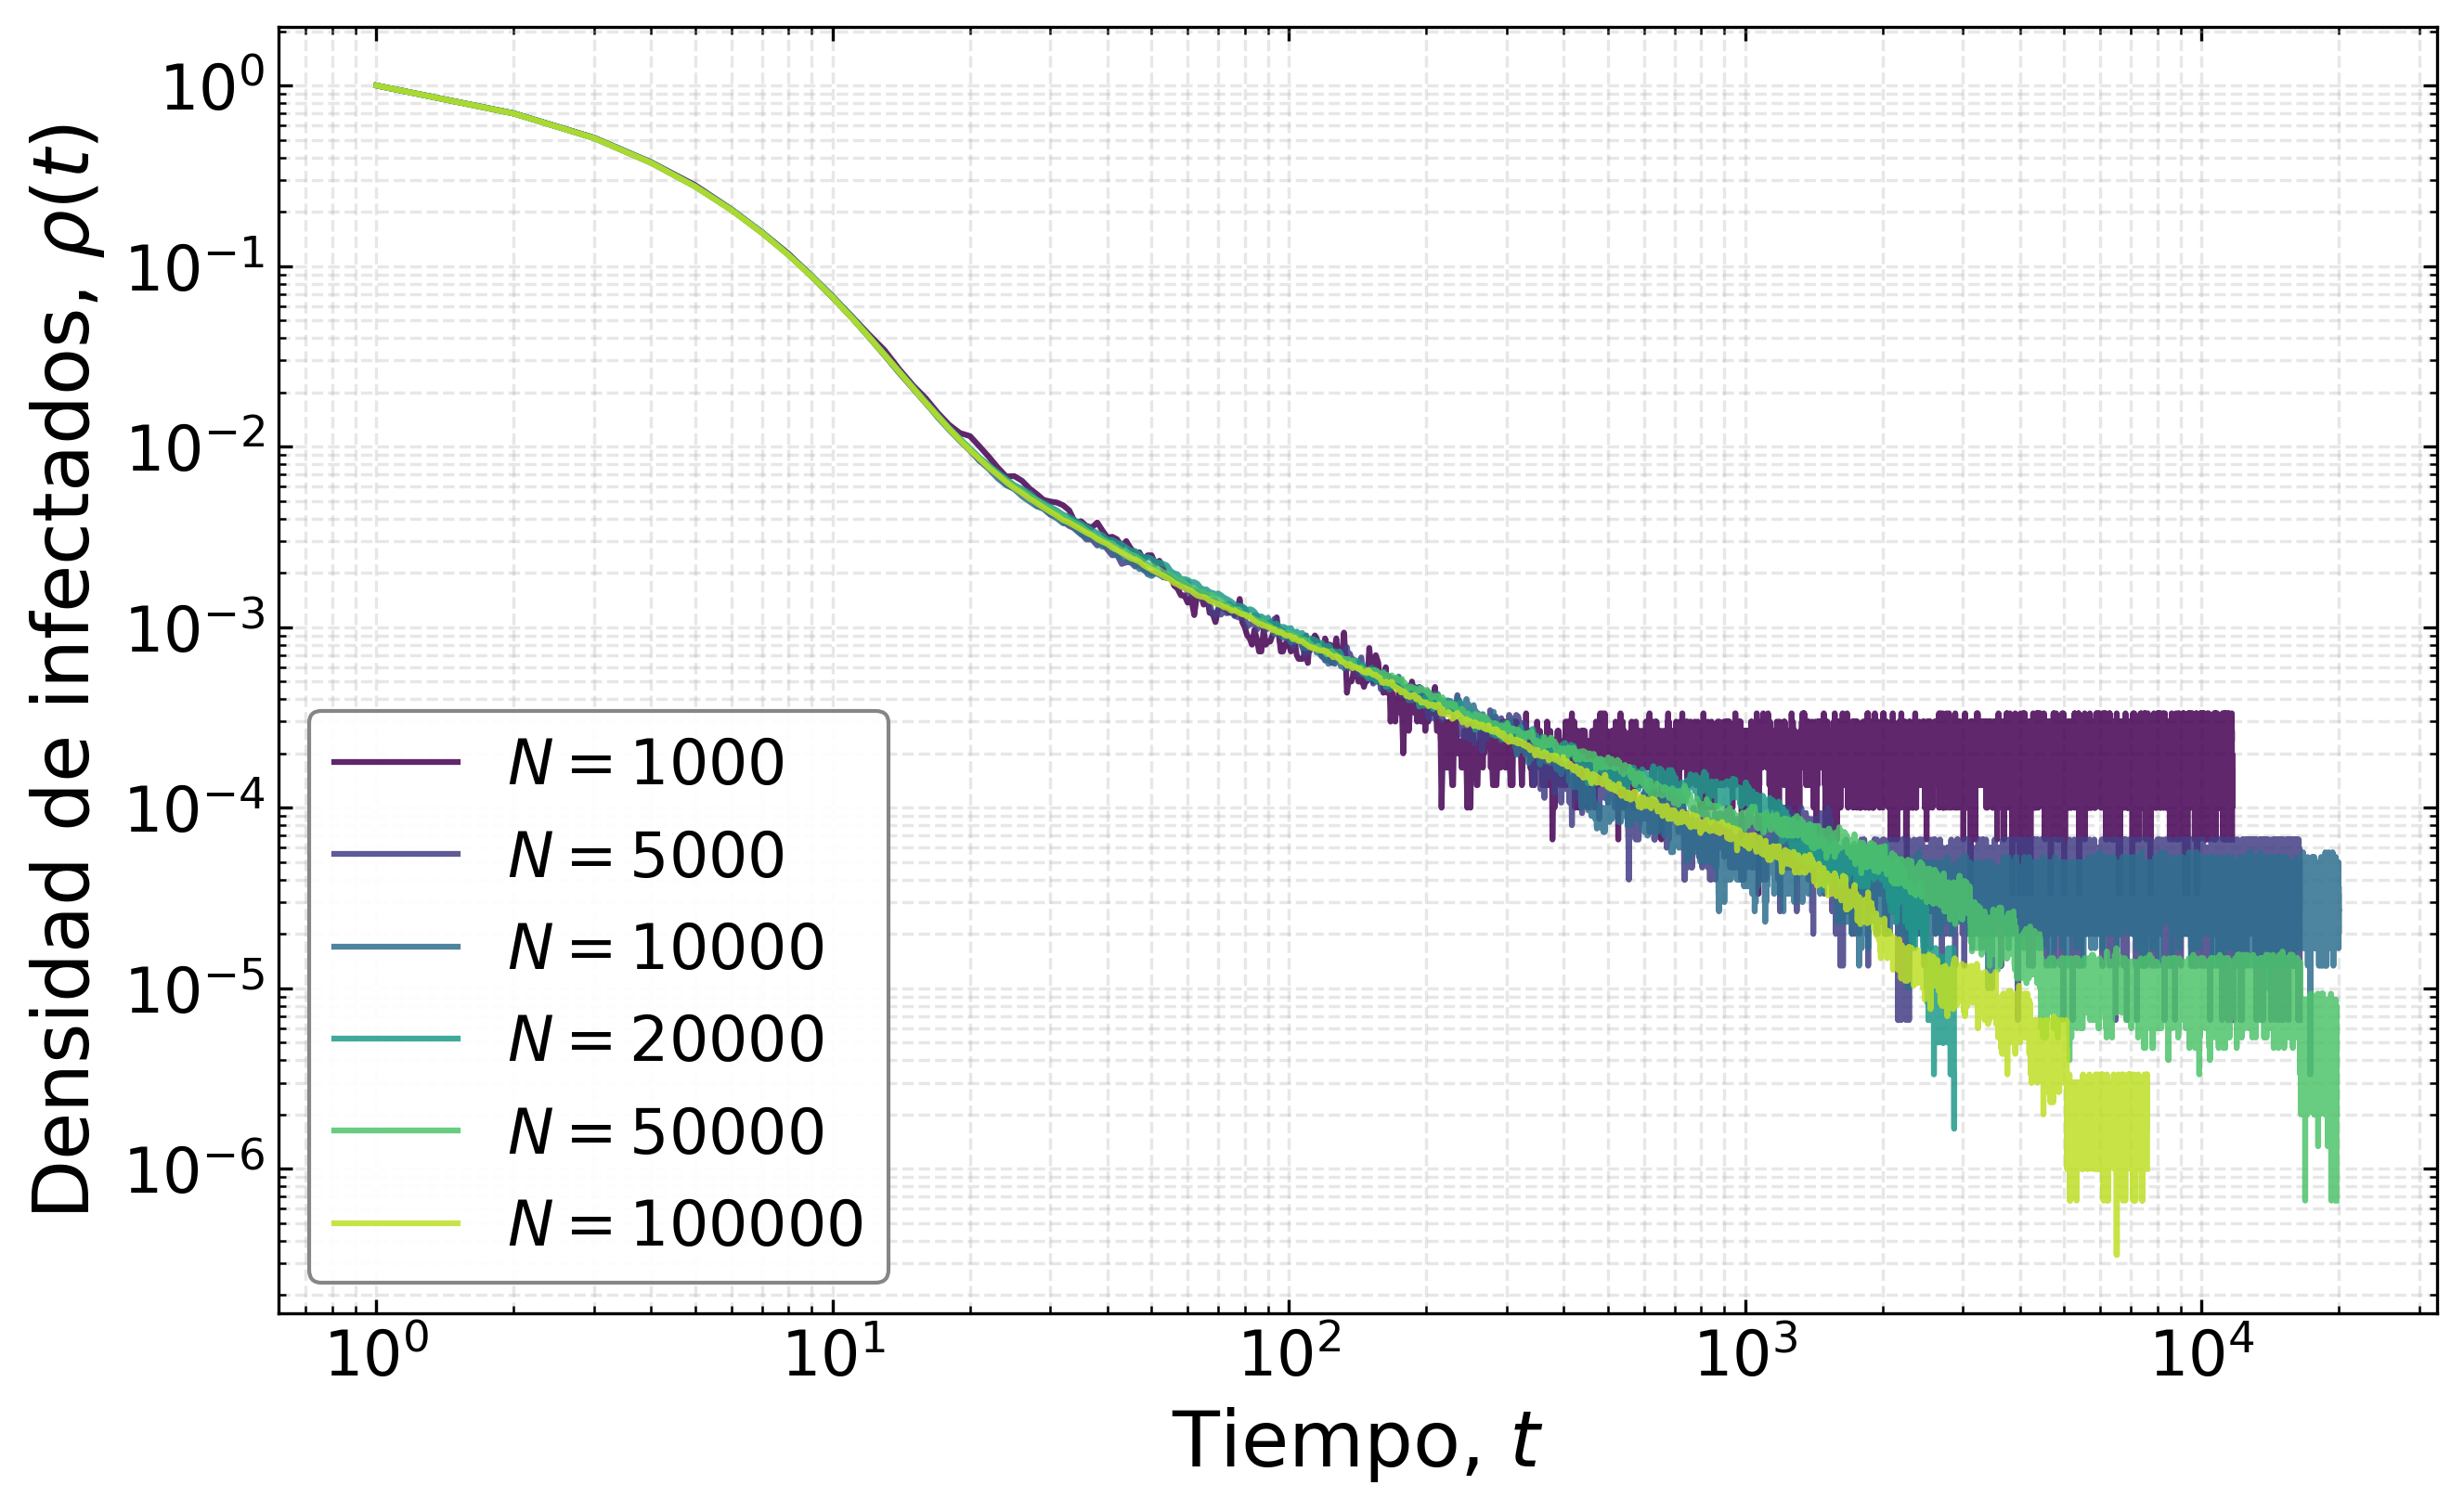
\includegraphics[width=0.9\columnwidth]{imagenes/1_griffiths_finite_size.png}
		\caption{Efectos de tamaño finito en la Fase de Griffiths ($q=0.90$, $\beta=0.60$). Las simulaciones para distintos tamaños de red $N$ muestran un colapso inicial sobre una misma ley de potencias, seguido de un truncamiento exponencial cuyo tiempo de inicio escala progresivamente con el tamaño del sistema.}
		\label{fig:finite_size}
	\end{figure}
	
	Adicionalmente, la finitud del sistema se manifiesta en el límite inferior de resolución de la densidad de infectados. Puesto que la población es discreta, la densidad mínima observable antes de la extinción total es $\rho_{min} = 1/N$ (en este estudio, $10^{-5}$). En las proximidades de la absorción, el número absoluto de individuos infectados fluctúa estocásticamente en valores microscópicos. Debido a la naturaleza de la representación logarítmica, estas fluctuaciones de escasas unidades se amplifican visualmente, generando una banda de ruido constante en el límite inferior de las curvas previo a la desaparición abrupta del patógeno, confirmando el carácter estocástico y discreto del proceso epidémico simulado.
	
	Finalmente, el análisis del punto marginal exacto ($q=q_{perc}=2/3$) se presenta en la Fig. \ref{fig:espectro_q_marginal}. En esta frontera geométrica, la distribución de tamaños de los clústeres activos pierde su cola exponencial y adopta una topología geométrica invariante de escala. Como consecuencia, tal y como predice la teoría, se produce un colapso del exponente algebraico ($\theta \to 0$), originando una dinámica de decaimiento logarítmico $\rho(t) \sim (\ln t)^{-1/2}$. Las simulaciones empíricas muestran curvas de relajación que, a diferencia de las rectas de la Fase de Griffiths, presentan una concavidad sostenida en escala logarítmica. La convergencia asintótica de los datos simulados con la curva teórica de referencia confirma que, en el umbral de percolación, la criticalidad topológica de la subred activa altera por completo la dinámica de la epidemia.
	
	\begin{figure}[htbp]
		\centering
		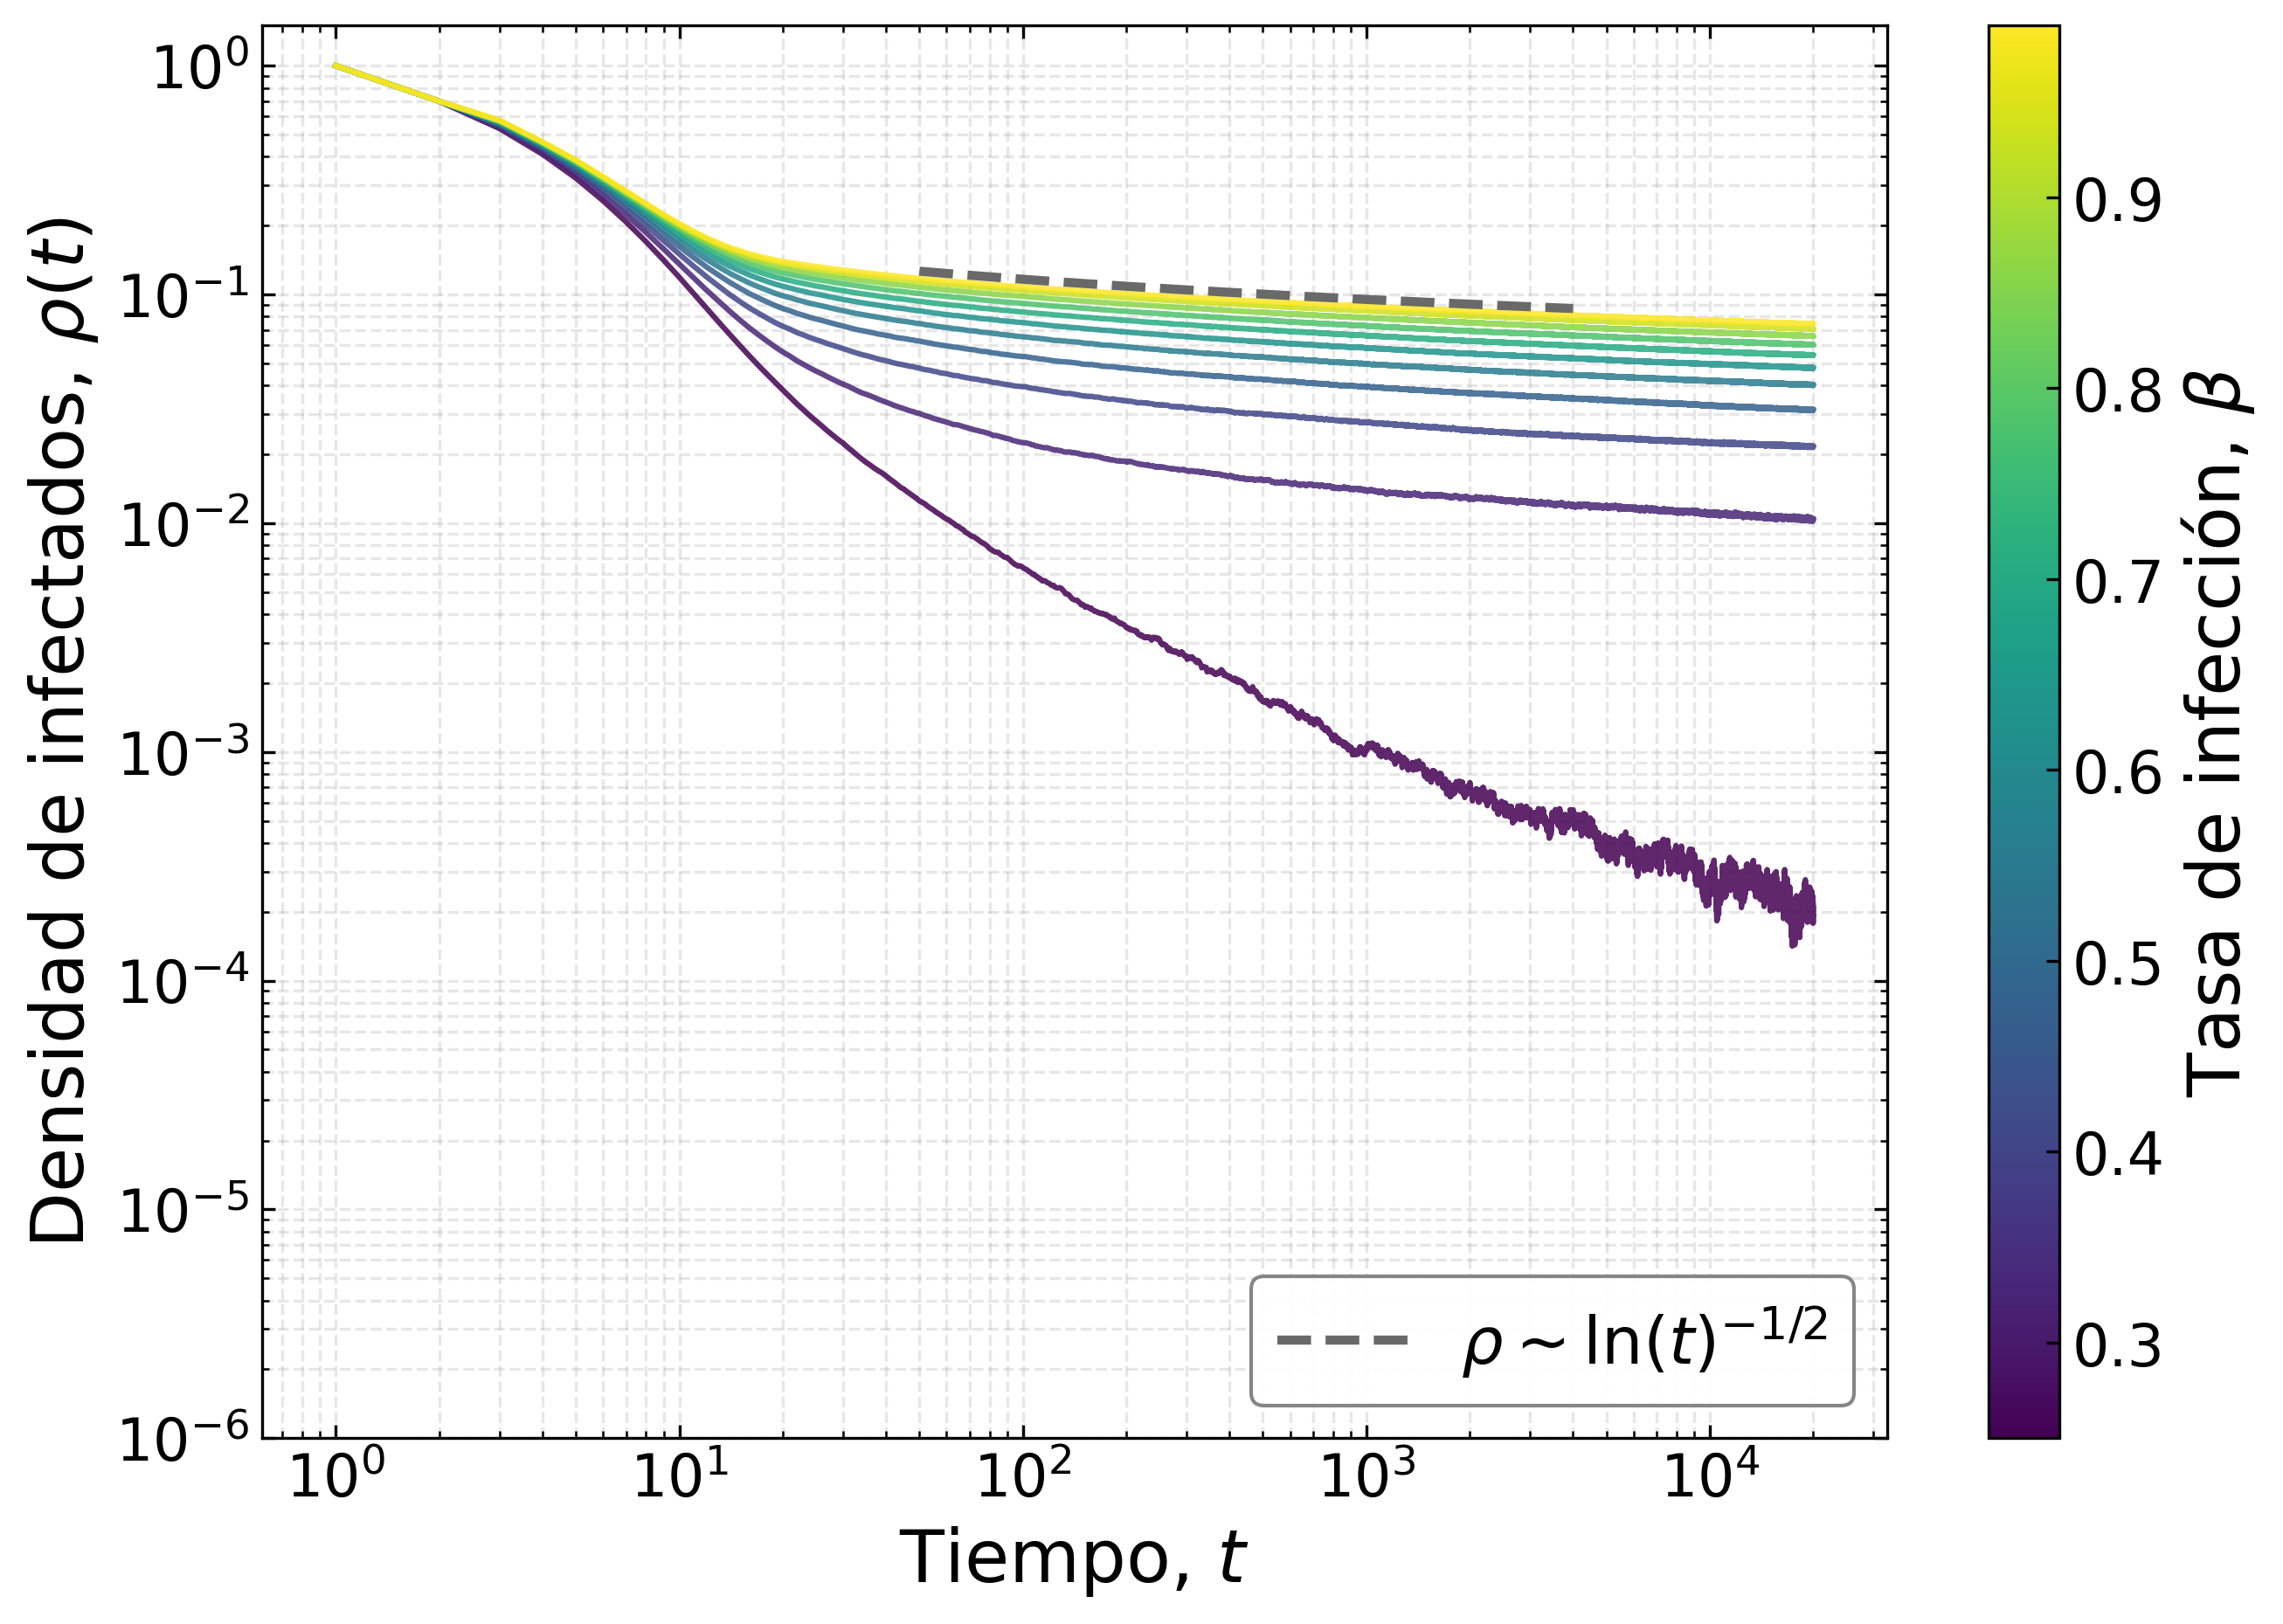
\includegraphics[width=0.9\columnwidth]{imagenes/summary_spectrum_q_2-3_selected.png}
		\caption{Espectro de relajación en la frontera de percolación marginal ($q = 2/3$). Las curvas exhiben el decaimiento logarítmico continuo característico de este régimen. La línea discontinua gris indica la función asintótica teórica $\rho(t) \sim (\ln t)^{-1/2}$.}
		\label{fig:espectro_q_marginal}
	\end{figure}
	
	En conjunto, los resultados de este estudio demuestran de manera inequívoca que la introducción de desorden estático en la red altera de manera fundamental la bifurcación clásica del modelo SIS. Al inducir la fragmentación topológica del sistema, el desorden da lugar a un escenario termodinámico dominado íntegramente por las fluctuaciones de las regiones raras. La aparición de la Fase de Griffiths, su dependencia con los efectos de tamaño finito y el régimen marginal logarítmico evidencian que, más allá de la tasa media de infección, la heterogeneidad y la distribución estadística extrema de las conexiones son los verdaderos mecanismos rectores de la dinámica epidémica macroscópica.
	
	\section{Conclusiones}
	En este trabajo se ha presentado un análisis sistemático sobre cómo la topología de las redes de interacción y la heterogeneidad estructural modifican las propiedades críticas de la propagación epidémica mediante el modelo SIS. Partiendo de una aproximación clásica de campo medio para un sistema bien mezclado, se ha transitado hacia la aproximación basada en el grado (DBMF) para capturar los efectos de la conectividad en redes complejas. Se ha demostrado analítica y numéricamente que la varianza de la distribución de grado subordina el umbral crítico, provocando su colapso hacia el origen en topologías de libre escala (Barabási-Albert). Para contextualizar la escala termodinámica de estas simulaciones, el tamaño máximo de red empleado ($N=500\,000$) es del mismo orden de magnitud que muchas poblaciones macroscópicas de áreas metropolitanas, como la de la ciudad de Granada. Esta equivalencia permite que los resultados obtenidos sean representativos de escenarios epidemiológicos con una escala demográfica y una complejidad urbana real.~\cite{PastorSatorras2015,Albert2002,Dorogovtsev2008}
	
	Por otro lado, la introducción de desorden estático (\textit{quenched disorder}) mediante una distribución bimodal de las tasas de infección ha revelado que la fragmentación topológica del sistema destruye el estado endémico global, dando paso a una región extensa de relajación anómala. En este régimen, la dinámica macroscópica queda dominada de forma absoluta por las fluctuaciones de las regiones raras, originando un espectro de fases absorbentes que abarca desde decaimientos exponenciales estirados hasta la invariancia de escala propia de la Fase de Griffiths, culminando en un decaimiento logarítmico marginal localizado exactamente sobre la frontera del umbral de percolación. Esta sección fue la más costosa de implementar. La convergencia de las simulaciones en el régimen fragmentado exige promediar sobre cientos de realizaciones del desorden, y los efectos de tamaño finito distorsionan sistemáticamente los umbrales teóricos. Esa discrepancia entre la predicción DBMF ($\beta \approx 0.225$) y el valor empírico ($\beta \gtrsim 0.45$) no es un error: es una consecuencia directa de las correlaciones locales que el campo medio ignora por construcción.
	
	Resulta fundamental contrastar empíricamente estos hallazgos con los resultados teóricos establecidos en la literatura física reciente. Otros estudios enfocados en modelos de propagación análogos, como el Proceso de Contacto (CP) evaluado bajo aproximaciones teóricas de pares, han predicho fenomenologías similares en redes aleatorias de Erdős-Rényi. Nuestro análisis numérico confirma de forma concluyente que, a pesar de emplear una dinámica de contagio iterativo diferente (SIS frente a CP) y basarnos en un marco analítico de red distinto (DBMF frente a la aproximación de pares), el abanico de regímenes anómalos emergentes es matemáticamente homólogo.~\cite{Muñoz2010,Noest1986,PastorSatorras2015,Odor2004} Este paralelismo subraya un principio de universalidad fundamental: la emergencia de la Fase de Griffiths no depende de los detalles microscópicos o locales de la transmisión de la enfermedad, sino que está dictada exclusivamente por la convolución subyacente entre la termodinámica de las fluctuaciones óptimas y la topología asintótica de las islas generadas por el desorden geométrico.
	
	Viendo todo esto, el resultado que más sorprende no es el colapso del umbral epidémico en redes de Barabási-Albert (eso lo predice la teoría), sino la robustez con la que la Fase de Griffiths sobrevive en simulaciones de tamaño finito. Aunque lo que se podría llegar a esperar en un principio es el desvanecimiento del régimen algebraico llegado a cierto punto de la simulación, con redes grandes ($N \sim 10^5$), se ha visto que esa tendencia ``recta'' (con forma de ley de potencias), se mantiene hasta llegar al límite físico impuesto por el tamaño finito de esta.
	
	Como resumen, este estudio constata que la heterogeneidad de grado y el desorden topológico no actúan como meras perturbaciones al modelo SIS clásico, sino como los verdaderos mecanismos rectores que alteran la clase de universalidad del sistema, dictando los tiempos de supervivencia del patógeno y redefiniendo por completo las fronteras de la criticidad epidémica. De alguna manera, el hecho de cambiar la red en la que se trabaja (no solo el modelo), cambia la física completamente, por lo que esta es una clara aplicación de como en un sistema es posible que ciertas propiedades macroscópicas emerjan solamente con un conjunto de relaciones de las propiedades microscópicas del mismo. ~\cite{PastorSatorras2015,Dorogovtsev2008,Muñoz2010,Noest1986,Odor2004}
	
	\section*{Disponibilidad de Código y Datos}
	El código fuente íntegro desarrollado para la ejecución de las simulaciones estocásticas, los cálculos analíticos, el tratamiento de datos espaciales y la generación de los diagramas de fases y espectros de relajación presentados en este trabajo, se encuentra publicado y accesible de forma abierta en el siguiente repositorio: \url{https://github.com/QuendoDev/SISModel}.
	
	
	% ==========================================
	% INICIO DE APÉNDICES
	% ==========================================
	
	
	\section{Apéndices}
	\subsection{La Ecuación Maestra}\label{apendice:mean_field}
	
	Sea $P(I, t)$ la probabilidad de que haya exactamente $I$ individuos infectados en el tiempo $t$. La Ecuación Maestra describe la evolución temporal de esta probabilidad:
	\begin{equation}
		\begin{split}
			\frac{dP(I,t)}{dt} ={} & W(I-1 \to I)P(I-1,t) \\
			& + W(I+1 \to I)P(I+1,t) \\
			& - W(I \to I+1)P(I,t) \\
			& - W(I \to I-1)P(I,t)
		\end{split}
	\end{equation}
	
	El cambio en la media, $\langle I \rangle = \sum_I I P(I, t)$, viene dado por:
	\begin{equation}
		\frac{d\langle I \rangle}{dt} = \langle W(I \to I+1) \rangle - \langle W(I \to I-1) \rangle
	\end{equation}
	
	Sustituyendo nuestras tasas de transición:
	\begin{equation}
		\frac{d\langle I \rangle}{dt} = \beta \langle I \rangle - \frac{\beta}{N} \langle I^2 \rangle - \mu \langle I \rangle
	\end{equation}
	
	En el límite termodinámico ($N \to \infty$), las fluctuaciones estocásticas se vuelven despreciables frente al tamaño del sistema.~\cite{PastorSatorras2015,Odor2004} Físicamente, esto implica que la varianza poblacional tiende a cero, justificando de manera rigurosa la aproximación de campo medio $\langle I^2 \rangle \approx \langle I \rangle^2$. Aplicando esta aproximación y dividiendo por la población total $N$, obtenemos la ecuación macroscópica en términos de la densidad $\rho(t) = \langle I \rangle / N$:
	\begin{equation}
		\frac{d\rho}{dt} = \beta \rho (1 - \rho) - \mu \rho
	\end{equation}
	
	\subsection{Derivación del umbral en redes heterogéneas (DBMF)}
	\label{apendice:dbmf}
	En una red sin correlaciones de grado, la probabilidad $\Theta$ de que un enlace apunte a un nodo infectado es independiente del grado del nodo origen y se calcula como:
	\begin{equation}
		\Theta = \frac{\sum_k (k-1) P(k) \rho_k}{\sum_k k P(k)} \approx \frac{1}{\langle k \rangle} \sum_k k P(k) \rho_k
	\end{equation}
	donde $P(k)$ es la probabilidad topológica de que un nodo de la red posea grado $k$.~\cite{Albert2002,Dorogovtsev2008,PastorSatorras2015}
	
	Buscamos el estado estacionario imponiendo la condición $d\rho_k/dt = 0$. Despejando $\rho_k$ de la ecuación de evolución, obtenemos:
	\begin{equation}
		\rho_k = \frac{\lambda k \Theta}{1 + \lambda k \Theta}
	\end{equation}
	donde hemos definido $\lambda = \beta/\mu$. Para que exista una solución endémica no trivial ($\rho_k > 0$), sustituimos esta expresión en la definición de $\Theta$. Para calcular el umbral crítico $\lambda_c$, analizamos el entorno de la transición de fase, donde la prevalencia es estadísticamente nula ($\rho_k \ll 1 \implies \Theta \ll 1$). En este límite asintótico, podemos linealizar el denominador empleando el primer término del desarrollo en serie de Taylor ($\frac{x}{1+x} \approx x$), lo que resulta en:
	\begin{equation}
		\Theta \approx \frac{1}{\langle k \rangle} \sum_k k P(k) (\lambda k \Theta) = \lambda \Theta \frac{\langle k^2 \rangle}{\langle k \rangle}
	\end{equation}
	donde se ha hecho uso de la definición estadística del segundo momento de la distribución de grado, $\langle k^2 \rangle = \sum_k k^2 P(k)$.~\cite{Albert2002,Dorogovtsev2008,PastorSatorras2015}
	
	Cancelando $\Theta$ a ambos lados de la igualdad, obtenemos la condición límite que define el umbral epidémico crítico:
	\begin{equation}
		\lambda_c = \frac{\langle k \rangle}{\langle k^2 \rangle}
	\end{equation}
	
	\subsection{Derivación del umbral DBMF para desorden bimodal en redes ER}
	\label{apendice:bimodal_dbmf}
	
	Consideremos una red sujeta a desorden bimodal donde una fracción $1-q$ de nodos (Tipo I) propaga la infección con tasa $\beta$, y la fracción $q$ (Tipo II) posee una tasa nula, fijando el parámetro de reducción a $r=0$.~\cite{Muñoz2010,PastorSatorras2015,Noest1986} A nivel macroscópico, basándonos en una formulación de campo medio simple (\textit{one-site mean-field}), la densidad global de infectados es la suma ponderada de ambas subpoblaciones: $\rho(t) = (1-q)\rho^I(t) + q\rho^{II}(t)$. Dado que los nodos Tipo II no pueden transmitir ni alojar la infección con efectividad, su contribución es nula ($\rho^{II}(t) = 0$), confinando la dinámica epidémica a la subred de Tipo I.
	
	Tomando como punto de partida la ecuación dinámica general DBMF para redes heterogéneas introducida previamente (Ec. \ref{ec:din_dbmf_het}), la evolución temporal de la densidad de infectados de grado $k$ pertenecientes al Tipo I se rige por:
	\begin{equation}
		\frac{d\rho_k^I(t)}{dt} = -\mu \rho_k^I(t) + \beta k [1 - \rho_k^I(t)] \Theta
	\end{equation}
	
	Para evaluar el inicio de la epidemia, evaluamos la estabilidad del sistema buscando el estado estacionario ($d\rho_k^I/dt = 0$), obteniendo:
	\begin{equation}
		\rho_k^I = \frac{(\beta/\mu) k \Theta}{1 + (\beta/\mu) k \Theta}
	\end{equation}
	
	La cantidad $\Theta$, que representa la probabilidad global de que un enlace elegido al azar apunte a un nodo infectado, debe estar estadísticamente ponderada por la fracción de la red capaz de sustentar la enfermedad:
	\begin{equation}
		\Theta = \frac{1-q}{\langle k \rangle} \sum_k k P(k) \rho_k^I
	\end{equation}
	
	Sustituyendo $\rho_k^I$ en esta expresión y linealizando el denominador en el límite de baja prevalencia $\Theta \to 0$, característico de la vecindad del punto crítico ($1 + (\beta/\mu) k \Theta \approx 1$), llegamos a:
	\begin{equation}
		\Theta \approx \frac{1-q}{\langle k \rangle} \sum_k k P(k) \left( \frac{\beta}{\mu} k \Theta \right)
	\end{equation}
	
	Recordando la definición del segundo momento de la distribución de grado, $\sum_k k^2 P(k) = \langle k^2 \rangle$, y cancelando $\Theta$ a ambos lados de la igualdad, hallamos el punto crítico general para una red bimodal:~\cite{Muñoz2010,PastorSatorras2015}
	\begin{equation}
		1 = (1-q) \frac{\beta_c}{\mu} \frac{\langle k^2 \rangle}{\langle k \rangle} \implies \beta_c(q) = \mu \frac{\langle k \rangle}{\langle k^2 \rangle} \frac{1}{1-q}
	\end{equation}
	
	Nótese que, en el límite de un sistema sin desorden ($q = 0$), esta expresión recupera de forma natural el umbral epidémico estándar para redes heterogéneas derivado en la Ec. \ref{eq:dbmf_threshold}. 
	
	Finalmente, particularizamos este resultado para la arquitectura específica de las redes aleatorias de Erdős-Rényi (ER) empleadas en nuestro estudio. En el límite termodinámico, la distribución de grado $P(k)$ de estas redes converge a una distribución de Poisson. Una propiedad fundamental de esta distribución es que su varianza $\sigma^2$ es estrictamente igual a su media $\langle k \rangle$.
	
	Aplicando la definición estadística de la varianza, $\sigma^2 = \langle k^2 \rangle - \langle k \rangle^2$, podemos expresar el segundo momento puramente en términos del grado medio:
	\begin{equation}
		\langle k^2 \rangle = \langle k \rangle^2 + \langle k \rangle = \langle k \rangle (\langle k \rangle + 1)
	\end{equation}
	
	Sustituyendo esta equivalencia topológica en la expresión general del umbral crítico obtenida, el grado medio en el numerador se cancela, arrojando la fórmula teórica definitiva para redes ER con desorden bimodal:
	\begin{equation}
		\beta_c^{DBMF}(q) = \mu \frac{\langle k \rangle}{\langle k \rangle (\langle k \rangle + 1)} \frac{1}{1-q} = \mu \frac{1}{\langle k \rangle + 1} \frac{1}{1-q}
	\end{equation}
	
	\subsection{Derivación del umbral de percolación en redes Erdős-Rényi}
	\label{apendice:percolacion}
	
	La introducción de nodos inactivos en la red puede modelarse matemáticamente como un proceso clásico de percolación de sitios (\textit{site percolation}).~\cite{Albert2002,Dorogovtsev2008} Consideremos una red de Erdős-Rényi original donde cada nodo posee, en promedio, $\langle k \rangle$ conexiones. Al ``apagar'' o silenciar una fracción $q$ de la población (nodos Tipo II), la topología efectiva queda restringida a una subred activa compuesta por la fracción restante de nodos, $p = 1 - q$.
	
	Dado que los nodos han sido eliminados de manera uniforme y aleatoria, la probabilidad de que un enlace original sobreviva (es decir, que conecte a dos nodos activos) es proporcional a la fracción de nodos que permanecen en el sistema. Por consiguiente, el nuevo grado medio de conectividad exclusivo entre los nodos de la subred activa (Tipo I) se reduce a:
	\begin{equation}
		\langle k_{activo} \rangle = p \langle k \rangle = (1 - q) \langle k \rangle
	\end{equation}
	
	Una propiedad topológica fundamental de las redes aleatorias de Erdős-Rényi establece que, para garantizar la existencia de una componente gigante conexa (una estructura macroscópica que abarque una fracción finita del sistema), el grado medio de la red debe ser estrictamente mayor que la unidad. Si $\langle k_{activo} \rangle \le 1$, la subred activa carece de la cohesión necesaria y se fragmenta ineludiblemente en una multiplicidad de clústeres finitos y aislados, impidiendo cualquier propagación epidémica a escala global.
	
	El punto crítico geométrico, que marca el límite exacto donde la componente gigante comienza a fragmentarse, se obtiene igualando el grado medio de la subred activa a la unidad:
	\begin{equation}
		\langle k_{activo} \rangle = 1 \implies (1 - q_{perc}) \langle k \rangle = 1
	\end{equation}
	
	Despejando analíticamente, hallamos el umbral crítico de percolación de sitios para este modelo:~\cite{Albert2002,Dorogovtsev2008}
	\begin{equation}
		q_{perc} = 1 - \frac{1}{\langle k \rangle}
	\end{equation}
	
	\subsection{Análisis Asintótico de las Fluctuaciones Óptimas}	
	\label{apendice:fluctuaciones}
	
	En el régimen fragmentado ($q \ge q_{perc}$), la red carece de componente gigante.~\cite{Albert2002,Dorogovtsev2008,Muñoz2010} Por tanto, la densidad total de infectados $\rho(t)$ puede aproximarse como la suma de la actividad independiente de múltiples ``islas'' o clústeres aislados de diversos tamaños $s$. Matemáticamente, esto se expresa como una integral sobre el espectro de tamaños:
	\begin{equation}
		\rho(t) \sim \int_{1}^{\infty} \mathcal{P}(s) \, e^{-t/\tau(s)} ds
	\end{equation}
	donde $\mathcal{P}(s)$ es la probabilidad topológica de hallar un clúster conexo de tamaño $s$, y $\tau(s)$ es el tiempo característico que la epidemia sobrevive en su interior. El comportamiento macroscópico del sistema emerge de la competición asintótica entre estas dos funciones, dando lugar a cuatro regímenes analíticos distintos:
	
	\subsubsection{Fase de Griffiths ($\beta > \beta_c(q_{perc})$ y $q > q_{perc}$)~\cite{Muñoz2010,Noest1986,Odor2004}}
	Al estar fragmentada la red, la teoría de percolación dicta que la distribución de clústeres decae exponencialmente. Para redes aleatorias de Erdős-Rényi, esta probabilidad topológica adopta la forma analítica $\mathcal{P}(s) \sim s^{-3/2} e^{-cs}$, donde la constante $c$ está unívocamente determinada por el grado medio de la subred activa $p = \langle k_{activo} \rangle = (1-q)\langle k \rangle$, cumpliendo $c = p - 1 - \ln(p)$. 
	
	Dado que $\beta$ es localmente supercrítico, el tiempo de vida en el interior de la isla crece exponencialmente con su tamaño: $\tau(s) \sim e^{As}$, con $A = A(\beta)$. Ignorando el factor algebraico subdominante, la integral resulta:
	\begin{equation}
		\rho(t) \sim \int ds \, \exp\left[ -c s - t e^{-A s} \right]
	\end{equation}
	En el límite asintótico ($t \to \infty$), evaluamos la integral mediante la aproximación de Laplace (punto silla). Buscamos el máximo del exponente $f(s) = -c s - t e^{-A s}$:
	\begin{equation}
		f'(s) = -c + t A e^{-A s} = 0 \implies s^* = \frac{1}{A} \ln\left(\frac{t A}{c}\right)
	\end{equation}
	Sustituyendo el punto óptimo $s^*$ en el término de decaimiento dominante $\exp(-c s^*)$, obtenemos el decaimiento algebraico genérico:
	\begin{equation}
		\rho(t) \sim t^{-c/A} = t^{-\frac{p - 1 - \ln(p)}{A(\beta)}} = t^{-\theta(q,\beta)}
	\end{equation}
	Esta expresión analítica para el exponente revela que cuando el sistema se aproxima al umbral de percolación ($q \to q_{perc}$), el grado medio activo tiende a la unidad ($p \to 1$). En este límite, la constante geométrica se anula ($c \to 0$), forzando matemáticamente a que $\theta \to 0$. Este colapso del exponente es el mecanismo responsable de destruir la ley de potencias, induciendo el cruce hacia el régimen logarítmico marginal.
	
	\subsubsection{Decaimiento Logarítmico Marginal ($q = q_{perc}$)~\cite{Muñoz2010,Noest1986,Odor2004}}
	En la frontera exacta de percolación, la estructura de las islas es un fractal estadístico y la cola exponencial de la probabilidad de clúster se desvanece ($c \to 0$), resultando en $\mathcal{P}(s) \sim s^{-3/2}$. Manteniendo $\tau(s) \sim e^{As}$, la integral es:
	\begin{equation}
		\rho(t) \sim \int ds \, s^{-3/2} \exp\left( -t e^{-A s} \right)
	\end{equation}
	Aplicando el cambio de variable $u = t e^{-A s}$, lo que implica $s = \frac{1}{A} \ln(t/u)$, la dependencia temporal dominante factoriza fuera de la integral, produciendo una relajación anómalamente lenta:
	\begin{equation}
		\rho(t) \sim (\ln t)^{-1/2}
	\end{equation}
	
	\subsubsection{Fase Exponencial Estirada ($\beta_c(0) < \beta < \beta_c(q_{perc})$)~\cite{Muñoz2010,Noest1986,Odor2004}}
	Si la tasa de infección es débil, las islas existen ($\mathcal{P}(s) \sim e^{-cs}$) pero el virus es dinámicamente subcrítico en su interior. En este caso, el tiempo de vida no crece exponencialmente, sino como una ley de potencias: $\tau(s) \sim s^z$. La integral toma la forma:
	\begin{equation}
		\rho(t) \sim \int ds \, \exp\left[ -c s - t s^{-z} \right]
	\end{equation}
	El nuevo punto silla para el exponente $f(s) = -cs - t s^{-z}$ ocurre en $s^* = (z t / c)^{\frac{1}{z+1}}$. Al sustituir este valor, surge el decaimiento exponencial estirado:
	\begin{equation}
		\rho(t) \sim \exp\left( -B \, t^{\frac{1}{z+1}} \right) = \exp\left( -B \, t^\alpha \right) \quad (\alpha < 1)
	\end{equation}
	
	\subsubsection{Fase Exponencial Pura ($\beta < \beta_c(0)$)~\cite{Muñoz2010,Noest1986,Odor2004}}
	Para tasas extremadamente débiles, la infección no posee la fuerza necesaria para propagarse por la topología de la isla. El tiempo de supervivencia se desacopla del tamaño del clúster y queda dictado puramente por la tasa de recuperación intrínseca: $\tau(s) \approx \tau_0 \approx 1/\mu$. En este caso, el término temporal es constante respecto a $s$ y sale de la integral:
	\begin{equation}
		\rho(t) \sim e^{-t/\tau_0} \int_{1}^{\infty} e^{-c s} ds = C \cdot e^{-t/\tau_0}
	\end{equation}
	recuperando de forma exacta el decaimiento exponencial clásico de los sistemas no correlacionados.
	
	\subsection{Clase de Universalidad de Percolación Dirigida en Campo Medio}
	\label{apendice:percolacion_dirigida}
	
	De acuerdo con la conjetura de Janssen-Grassberger, las transiciones de fase continuas hacia un estado absorbente único en sistemas sin simetrías adicionales pertenecen genéricamente a la clase de universalidad de la Percolación Dirigida (DP).~\cite{Noest1986,Odor2004} Las redes de Erdős-Rényi y Watts-Strogatz empleadas en este estudio poseen una dimensión topológica infinita ($D \to \infty$), lo que las sitúa muy por encima de la dimensión crítica superior de la DP ($d_c = 4$).
	
	En este régimen termodinámico, las fluctuaciones espaciales locales se vuelven irrelevantes y los exponentes críticos del sistema convergen de manera exacta a los valores predichos por la teoría de campo medio. Matemáticamente, el crecimiento del parámetro de orden en el estado estacionario por encima del punto crítico está gobernado por el exponente estático $\alpha$ (denotado como $\beta$ en la literatura de física estadística), cuyo valor analítico en campo medio es unitario ($\alpha = 1$). 
	
	De forma análoga, la relajación dinámica de la densidad de infectados evaluada exactamente sobre la frontera crítica obedece una ley de potencias $\rho(t) \sim t^{-\delta}$, caracterizada por el exponente dinámico temporal. En el límite de campo medio, este exponente dinámico adopta igualmente un valor unitario ($\delta = 1$). Estas predicciones universales constituyen el marco teórico fundamental sobre el que se validan empíricamente los exponentes extraídos mediante escalamiento computacional.~\cite{Odor2004,Noest1986}
	
	\bibliography{apssamp}
	
\end{document}
% ****** End of file apssamp.tex ******